% Options for packages loaded elsewhere
\PassOptionsToPackage{unicode}{hyperref}
\PassOptionsToPackage{hyphens}{url}
\PassOptionsToPackage{dvipsnames,svgnames,x11names}{xcolor}
%
\documentclass[
  a4paper,
  DIV=11]{scrreprt}

\usepackage{amsmath,amssymb}
\usepackage{iftex}
\ifPDFTeX
  \usepackage[T1]{fontenc}
  \usepackage[utf8]{inputenc}
  \usepackage{textcomp} % provide euro and other symbols
\else % if luatex or xetex
  \usepackage{unicode-math}
  \defaultfontfeatures{Scale=MatchLowercase}
  \defaultfontfeatures[\rmfamily]{Ligatures=TeX,Scale=1}
\fi
\usepackage{lmodern}
\ifPDFTeX\else  
    % xetex/luatex font selection
    \setmainfont[]{Times New Roman}
    \setsansfont[]{Arial}
    \setmonofont[]{Courier New}
\fi
% Use upquote if available, for straight quotes in verbatim environments
\IfFileExists{upquote.sty}{\usepackage{upquote}}{}
\IfFileExists{microtype.sty}{% use microtype if available
  \usepackage[]{microtype}
  \UseMicrotypeSet[protrusion]{basicmath} % disable protrusion for tt fonts
}{}
\makeatletter
\@ifundefined{KOMAClassName}{% if non-KOMA class
  \IfFileExists{parskip.sty}{%
    \usepackage{parskip}
  }{% else
    \setlength{\parindent}{0pt}
    \setlength{\parskip}{6pt plus 2pt minus 1pt}}
}{% if KOMA class
  \KOMAoptions{parskip=half}}
\makeatother
\usepackage{xcolor}
\setlength{\emergencystretch}{3em} % prevent overfull lines
\setcounter{secnumdepth}{5}
% Make \paragraph and \subparagraph free-standing
\makeatletter
\ifx\paragraph\undefined\else
  \let\oldparagraph\paragraph
  \renewcommand{\paragraph}{
    \@ifstar
      \xxxParagraphStar
      \xxxParagraphNoStar
  }
  \newcommand{\xxxParagraphStar}[1]{\oldparagraph*{#1}\mbox{}}
  \newcommand{\xxxParagraphNoStar}[1]{\oldparagraph{#1}\mbox{}}
\fi
\ifx\subparagraph\undefined\else
  \let\oldsubparagraph\subparagraph
  \renewcommand{\subparagraph}{
    \@ifstar
      \xxxSubParagraphStar
      \xxxSubParagraphNoStar
  }
  \newcommand{\xxxSubParagraphStar}[1]{\oldsubparagraph*{#1}\mbox{}}
  \newcommand{\xxxSubParagraphNoStar}[1]{\oldsubparagraph{#1}\mbox{}}
\fi
\makeatother

\usepackage{color}
\usepackage{fancyvrb}
\newcommand{\VerbBar}{|}
\newcommand{\VERB}{\Verb[commandchars=\\\{\}]}
\DefineVerbatimEnvironment{Highlighting}{Verbatim}{commandchars=\\\{\}}
% Add ',fontsize=\small' for more characters per line
\usepackage{framed}
\definecolor{shadecolor}{RGB}{241,243,245}
\newenvironment{Shaded}{\begin{snugshade}}{\end{snugshade}}
\newcommand{\AlertTok}[1]{\textcolor[rgb]{0.68,0.00,0.00}{#1}}
\newcommand{\AnnotationTok}[1]{\textcolor[rgb]{0.37,0.37,0.37}{#1}}
\newcommand{\AttributeTok}[1]{\textcolor[rgb]{0.40,0.45,0.13}{#1}}
\newcommand{\BaseNTok}[1]{\textcolor[rgb]{0.68,0.00,0.00}{#1}}
\newcommand{\BuiltInTok}[1]{\textcolor[rgb]{0.00,0.23,0.31}{#1}}
\newcommand{\CharTok}[1]{\textcolor[rgb]{0.13,0.47,0.30}{#1}}
\newcommand{\CommentTok}[1]{\textcolor[rgb]{0.37,0.37,0.37}{#1}}
\newcommand{\CommentVarTok}[1]{\textcolor[rgb]{0.37,0.37,0.37}{\textit{#1}}}
\newcommand{\ConstantTok}[1]{\textcolor[rgb]{0.56,0.35,0.01}{#1}}
\newcommand{\ControlFlowTok}[1]{\textcolor[rgb]{0.00,0.23,0.31}{\textbf{#1}}}
\newcommand{\DataTypeTok}[1]{\textcolor[rgb]{0.68,0.00,0.00}{#1}}
\newcommand{\DecValTok}[1]{\textcolor[rgb]{0.68,0.00,0.00}{#1}}
\newcommand{\DocumentationTok}[1]{\textcolor[rgb]{0.37,0.37,0.37}{\textit{#1}}}
\newcommand{\ErrorTok}[1]{\textcolor[rgb]{0.68,0.00,0.00}{#1}}
\newcommand{\ExtensionTok}[1]{\textcolor[rgb]{0.00,0.23,0.31}{#1}}
\newcommand{\FloatTok}[1]{\textcolor[rgb]{0.68,0.00,0.00}{#1}}
\newcommand{\FunctionTok}[1]{\textcolor[rgb]{0.28,0.35,0.67}{#1}}
\newcommand{\ImportTok}[1]{\textcolor[rgb]{0.00,0.46,0.62}{#1}}
\newcommand{\InformationTok}[1]{\textcolor[rgb]{0.37,0.37,0.37}{#1}}
\newcommand{\KeywordTok}[1]{\textcolor[rgb]{0.00,0.23,0.31}{\textbf{#1}}}
\newcommand{\NormalTok}[1]{\textcolor[rgb]{0.00,0.23,0.31}{#1}}
\newcommand{\OperatorTok}[1]{\textcolor[rgb]{0.37,0.37,0.37}{#1}}
\newcommand{\OtherTok}[1]{\textcolor[rgb]{0.00,0.23,0.31}{#1}}
\newcommand{\PreprocessorTok}[1]{\textcolor[rgb]{0.68,0.00,0.00}{#1}}
\newcommand{\RegionMarkerTok}[1]{\textcolor[rgb]{0.00,0.23,0.31}{#1}}
\newcommand{\SpecialCharTok}[1]{\textcolor[rgb]{0.37,0.37,0.37}{#1}}
\newcommand{\SpecialStringTok}[1]{\textcolor[rgb]{0.13,0.47,0.30}{#1}}
\newcommand{\StringTok}[1]{\textcolor[rgb]{0.13,0.47,0.30}{#1}}
\newcommand{\VariableTok}[1]{\textcolor[rgb]{0.07,0.07,0.07}{#1}}
\newcommand{\VerbatimStringTok}[1]{\textcolor[rgb]{0.13,0.47,0.30}{#1}}
\newcommand{\WarningTok}[1]{\textcolor[rgb]{0.37,0.37,0.37}{\textit{#1}}}

\providecommand{\tightlist}{%
  \setlength{\itemsep}{0pt}\setlength{\parskip}{0pt}}\usepackage{longtable,booktabs,array}
\usepackage{calc} % for calculating minipage widths
% Correct order of tables after \paragraph or \subparagraph
\usepackage{etoolbox}
\makeatletter
\patchcmd\longtable{\par}{\if@noskipsec\mbox{}\fi\par}{}{}
\makeatother
% Allow footnotes in longtable head/foot
\IfFileExists{footnotehyper.sty}{\usepackage{footnotehyper}}{\usepackage{footnote}}
\makesavenoteenv{longtable}
\usepackage{graphicx}
\makeatletter
\def\maxwidth{\ifdim\Gin@nat@width>\linewidth\linewidth\else\Gin@nat@width\fi}
\def\maxheight{\ifdim\Gin@nat@height>\textheight\textheight\else\Gin@nat@height\fi}
\makeatother
% Scale images if necessary, so that they will not overflow the page
% margins by default, and it is still possible to overwrite the defaults
% using explicit options in \includegraphics[width, height, ...]{}
\setkeys{Gin}{width=\maxwidth,height=\maxheight,keepaspectratio}
% Set default figure placement to htbp
\makeatletter
\def\fps@figure{htbp}
\makeatother
% definitions for citeproc citations
\NewDocumentCommand\citeproctext{}{}
\NewDocumentCommand\citeproc{mm}{%
  \begingroup\def\citeproctext{#2}\cite{#1}\endgroup}
\makeatletter
 % allow citations to break across lines
 \let\@cite@ofmt\@firstofone
 % avoid brackets around text for \cite:
 \def\@biblabel#1{}
 \def\@cite#1#2{{#1\if@tempswa , #2\fi}}
\makeatother
\newlength{\cslhangindent}
\setlength{\cslhangindent}{1.5em}
\newlength{\csllabelwidth}
\setlength{\csllabelwidth}{3em}
\newenvironment{CSLReferences}[2] % #1 hanging-indent, #2 entry-spacing
 {\begin{list}{}{%
  \setlength{\itemindent}{0pt}
  \setlength{\leftmargin}{0pt}
  \setlength{\parsep}{0pt}
  % turn on hanging indent if param 1 is 1
  \ifodd #1
   \setlength{\leftmargin}{\cslhangindent}
   \setlength{\itemindent}{-1\cslhangindent}
  \fi
  % set entry spacing
  \setlength{\itemsep}{#2\baselineskip}}}
 {\end{list}}
\usepackage{calc}
\newcommand{\CSLBlock}[1]{\hfill\break\parbox[t]{\linewidth}{\strut\ignorespaces#1\strut}}
\newcommand{\CSLLeftMargin}[1]{\parbox[t]{\csllabelwidth}{\strut#1\strut}}
\newcommand{\CSLRightInline}[1]{\parbox[t]{\linewidth - \csllabelwidth}{\strut#1\strut}}
\newcommand{\CSLIndent}[1]{\hspace{\cslhangindent}#1}

% load packages
%\usepackage{multicol}
\usepackage{fontspec}
\usepackage{emoji}
\usepackage{xltxtra}
%\usepackage{xcolor}
\usepackage{listings}
\usepackage{fvextra}


\definecolor{ycol}{RGB}{230,159,0}
\definecolor{modelcol}{RGB}{86,180,233}
\definecolor{errorcol}{RGB}{0,158,115}
\definecolor{beta0col}{RGB}{213,94,0}
\definecolor{beta1col}{RGB}{0,114,178}
\definecolor{xcol}{RGB}{204,121,167}


\lstset{
  breaklines=true
}

\DefineVerbatimEnvironment{Highlighting}{Verbatim}{breaklines,commandchars=\\\{\}}
\DefineVerbatimEnvironment{OutputCode}{Verbatim}{breaklines,commandchars=\\\{\}}
\KOMAoption{captions}{tableheading}
\makeatletter
\@ifpackageloaded{tcolorbox}{}{\usepackage[skins,breakable]{tcolorbox}}
\@ifpackageloaded{fontawesome5}{}{\usepackage{fontawesome5}}
\definecolor{quarto-callout-color}{HTML}{909090}
\definecolor{quarto-callout-note-color}{HTML}{0758E5}
\definecolor{quarto-callout-important-color}{HTML}{CC1914}
\definecolor{quarto-callout-warning-color}{HTML}{EB9113}
\definecolor{quarto-callout-tip-color}{HTML}{00A047}
\definecolor{quarto-callout-caution-color}{HTML}{FC5300}
\definecolor{quarto-callout-color-frame}{HTML}{acacac}
\definecolor{quarto-callout-note-color-frame}{HTML}{4582ec}
\definecolor{quarto-callout-important-color-frame}{HTML}{d9534f}
\definecolor{quarto-callout-warning-color-frame}{HTML}{f0ad4e}
\definecolor{quarto-callout-tip-color-frame}{HTML}{02b875}
\definecolor{quarto-callout-caution-color-frame}{HTML}{fd7e14}
\makeatother
\makeatletter
\@ifpackageloaded{caption}{}{\usepackage{caption}}
\AtBeginDocument{%
\ifdefined\contentsname
  \renewcommand*\contentsname{Inhaltsverzeichnis}
\else
  \newcommand\contentsname{Inhaltsverzeichnis}
\fi
\ifdefined\listfigurename
  \renewcommand*\listfigurename{Abbildungsverzeichnis}
\else
  \newcommand\listfigurename{Abbildungsverzeichnis}
\fi
\ifdefined\listtablename
  \renewcommand*\listtablename{Tabellenverzeichnis}
\else
  \newcommand\listtablename{Tabellenverzeichnis}
\fi
\ifdefined\figurename
  \renewcommand*\figurename{Abbildung}
\else
  \newcommand\figurename{Abbildung}
\fi
\ifdefined\tablename
  \renewcommand*\tablename{Tabelle}
\else
  \newcommand\tablename{Tabelle}
\fi
}
\@ifpackageloaded{float}{}{\usepackage{float}}
\floatstyle{ruled}
\@ifundefined{c@chapter}{\newfloat{codelisting}{h}{lop}}{\newfloat{codelisting}{h}{lop}[chapter]}
\floatname{codelisting}{Listing}
\newcommand*\listoflistings{\listof{codelisting}{Listingverzeichnis}}
\usepackage{amsthm}
\theoremstyle{definition}
\newtheorem{exercise}{Übungsaufgabe}[chapter]
\theoremstyle{definition}
\newtheorem{definition}{Definition}[chapter]
\theoremstyle{definition}
\newtheorem{example}{Beispiel}[chapter]
\theoremstyle{remark}
\AtBeginDocument{\renewcommand*{\proofname}{Beweis}}
\newtheorem*{remark}{Anmerkung}
\newtheorem*{solution}{Lösung}
\newtheorem{refremark}{Anmerkung}[chapter]
\newtheorem{refsolution}{Lösung}[chapter]
\makeatother
\makeatletter
\makeatother
\makeatletter
\@ifpackageloaded{caption}{}{\usepackage{caption}}
\@ifpackageloaded{subcaption}{}{\usepackage{subcaption}}
\makeatother

\ifLuaTeX
\usepackage[bidi=basic]{babel}
\else
\usepackage[bidi=default]{babel}
\fi
\babelprovide[main,import]{ngerman}
\ifPDFTeX
\else
\babelfont{rm}[]{Times New Roman}
\fi
% get rid of language-specific shorthands (see #6817):
\let\LanguageShortHands\languageshorthands
\def\languageshorthands#1{}
\ifLuaTeX
  \usepackage{selnolig}  % disable illegal ligatures
\fi
\usepackage{bookmark}

\IfFileExists{xurl.sty}{\usepackage{xurl}}{} % add URL line breaks if available
\urlstyle{same} % disable monospaced font for URLs
\hypersetup{
  pdftitle={Statistik1},
  pdfauthor={Sebastian Sauer},
  pdflang={de},
  colorlinks=true,
  linkcolor={blue},
  filecolor={Maroon},
  citecolor={Blue},
  urlcolor={Blue},
  pdfcreator={LaTeX via pandoc}}


\title{Statistik1}
\author{Sebastian Sauer}
\date{2024-08-29}

\begin{document}
\maketitle

\renewcommand*\contentsname{Inhaltsverzeichnis}
{
\hypersetup{linkcolor=}
\setcounter{tocdepth}{2}
\tableofcontents
}

\chapter{Willkommen!}\label{willkommen}

\begin{figure}[H]

{\centering 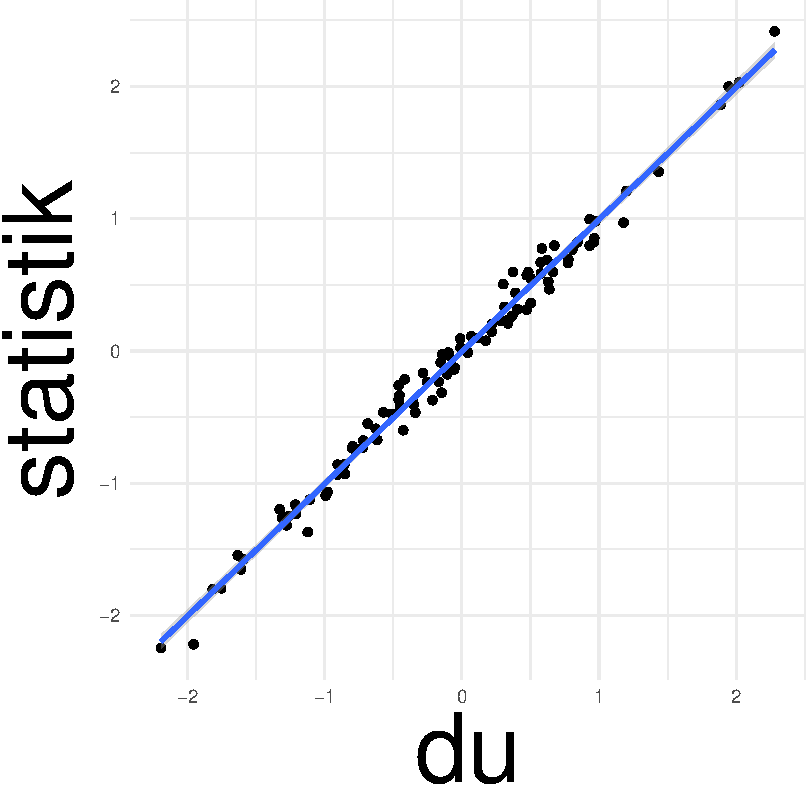
\includegraphics[width=0.33\textwidth,height=\textheight]{index_files/figure-pdf/unnamed-chunk-1-1.pdf}

}

\caption{Statistik und Du: Guter Fit!}

\end{figure}%

\section{Es geht um Ihren Lernerfolg}\label{es-geht-um-ihren-lernerfolg}

Meister Yoda rät: Lesen Sie die Hinweise (Abbildung~\ref{fig-yoda}).

\begin{figure}

\centering{


\includegraphics[width=0.5\textwidth,height=\textheight]{img/yoda.jpg}

}

\caption{\label{fig-yoda}Lesen Sie die folgenden Hinweise im eigenen
Interesse}

\end{figure}%

\href{https://imgflip.com/memegenerator}{Quelle: Imgflip Memengenerator}

\subsection{Lernziele}\label{lernziele}

\begin{itemize}
\item
  Die Studentis sind mit wesentlichen Methoden der explorativen
  Datenanalyse vertraut und können diese selbständig anwenden.
\item
  Die Studentis können gängige Forschungsfragen in lineare Modelle
  übersetzen, diese auf echte Datensätze anwenden und die Ergebnisse
  interpretieren.
\end{itemize}

Kurz gesagt: Das ist ein Grundkurs in Daten zähmen.

\begin{figure}[H]

{\centering 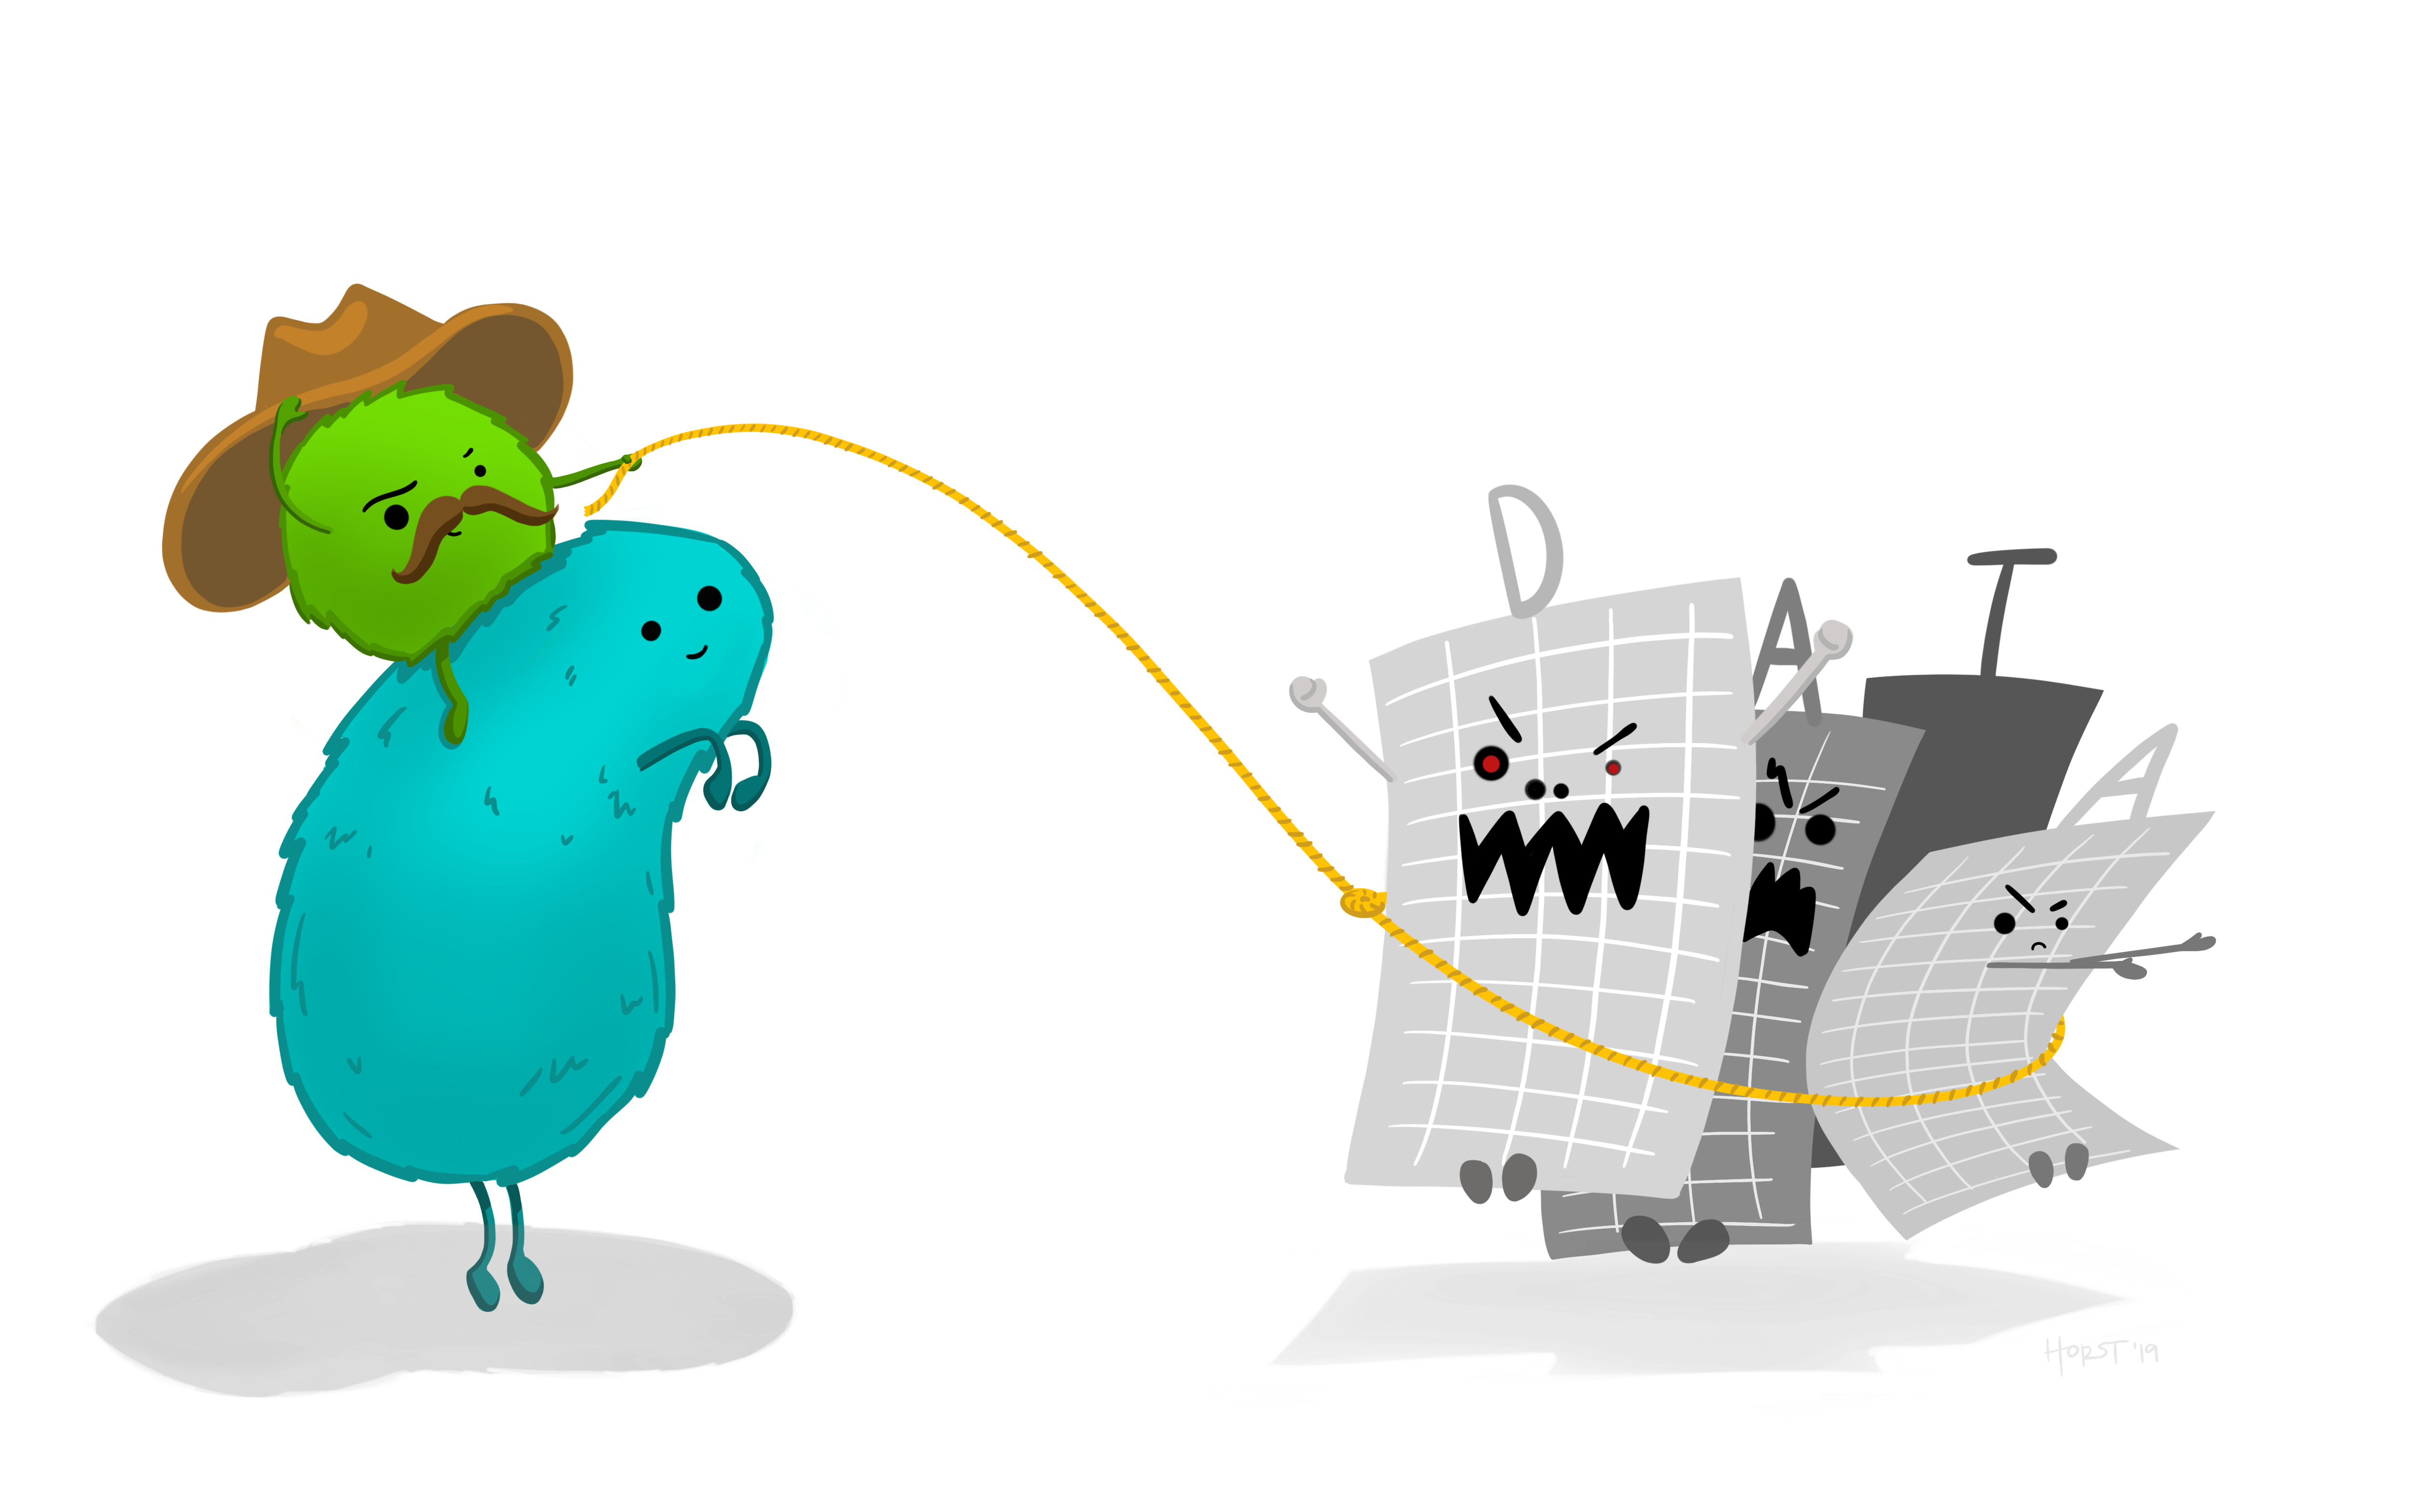
\includegraphics[width=0.5\textwidth,height=\textheight]{img/datenzaehmen.png}

}

\caption{Daten zähmen}

\end{figure}%

\href{https://github.com/allisonhorst/stats-illustrations}{Bildquelle:
Allison Horst, CC-BY}

\subsection{Was lerne ich hier und wozu ist das
gut?}\label{was-lerne-ich-hier-und-wozu-ist-das-gut}

\emph{Was lerne ich hier?}

Sie lernen das \emph{Handwerk der Datenanalyse} mit einem Schwerpunkt
auf Vorhersage. Anders gesagt: Sie lernen, \emph{Daten aufzubereiten}
und aus Daten \emph{Vorhersagen} abzuleiten. Zum Beispiel: Kommt ein
Student zu Ihnen und sagt ``Ich habe 42 Stunden für die Klausur gelernt,
welche Note kann ich in der Klausur erwarten?''. Darauf Ihre Antwort:
``Auf Basis meiner Daten und meines Modells müsstest du eine 2.7
schreiben!''.\footnote{Darauf dis Studenti: ``Hpmf.''}. Außerdem lernen
Sie, wie man die Güte einer Vorhersage auf Stichhaltigkeit prüft. Denn
Vorhersagen kann man ja in jeder Eckkneipe oder beim Wahrsager bekommen.
Wir wollen aber belastbare Vorhersagen und zumindest wissen, wie gut die
Vorhersagen (von jemanden) bisher waren.

\emph{Warum ist das wichtig?}

Wir wollen nicht auf Leuten vertrauen, die behaupten, sie wüssten, was
für uns richtig und gut ist. Wir wollen selber die Fakten prüfen können.

\emph{Wozu brauche ich das im Job?}

Datenanalyse spielt bereits heute in vielen Berufen eine Rolle. Tendenz
stark zunehmend.

\emph{Wozu brauche ich das im weiterem Studium?}

In Forschungsarbeiten (wie in empirischen Forschungsprojekten, etwa in
der Abschlussarbeit) ist es üblich, statistische Ergebnisse hinsichtlich
quantitativ zu analysieren.

\emph{Ist Statistik nicht sehr abstrakt?}

Der Schwerpunkt dieses Kurses liegt auf Anwenden und Tun; ähnlich dem
Erlernen eines Handwerks. Theorien und Abstraktionen stehen nur am Rand.

\emph{Gibt es auch gute Jobs, wenn man sich mit Daten auskennt?}

Das Forum (2020) berichtet zu den ``Top 20 job roles in increasing and
decreasing demand across industries'' (S. 30, Abb. 22):

\begin{enumerate}
\def\labelenumi{\arabic{enumi}.}
\tightlist
\item
  Data Analysts und Scientists
\item
  AI and Machine Learning Specialists
\item
  Big Data Specialists
\end{enumerate}

\subsection{Was ist hier das
Erfolgsgeheimnis?}\label{was-ist-hier-das-erfolgsgeheimnis}

\begin{tcolorbox}[enhanced jigsaw, opacityback=0, arc=.35mm, left=2mm, colframe=quarto-callout-important-color-frame, toptitle=1mm, colback=white, toprule=.15mm, bottomrule=.15mm, colbacktitle=quarto-callout-important-color!10!white, bottomtitle=1mm, coltitle=black, titlerule=0mm, title=\textcolor{quarto-callout-important-color}{\faExclamation}\hspace{0.5em}{Wichtig}, rightrule=.15mm, breakable, leftrule=.75mm, opacitybacktitle=0.6]

\emph{Dran bleiben} ist der Schlüssel zum Erfolg. Üben Sie regelmäßig.
Geben Sie bei Schwierigkeiten nicht auf.

\emoji{person-lifting-weights} \emoji{clockwise-vertical-arrows}
\emoji{key} \emoji{glowing-star} \(\square\)

\end{tcolorbox}

\subsection{Motivieren Sie mich!}\label{motivieren-sie-mich}

Schauen Sie sich das Video mit einer
\href{https://youtu.be/jtNlzpcPr5Y}{Ansprache zur Motivation}
an.\footnote{\url{https://youtu.be/jtNlzpcPr5Y}}

\subsection{Voraussetzungen}\label{voraussetzungen}

Um von diesem Kurs am besten zu profitieren, sollten Sie Folgendes
mitbringen:

\begin{itemize}
\tightlist
\item
  Bereitschaft, Neues zu lernen
\item
  Bereitschaft, nicht gleich aufzugeben
\item
  Kenntnis grundlegender Methoden wissenschaftlichen Arbeitens
\end{itemize}

Was Sie \emph{nicht} brauchen, sind besondere Mathe-Vorkenntnisse.

\subsection{Überblick}\label{uxfcberblick}

Abb. Abbildung~\ref{fig-ueberblick} gibt einen Überblick über den
Verlauf und die Inhalte des Buches. Das Diagramm hilft Ihnen zu
verorten, wo welches Thema im Gesamtzusammenhang steht.

\begin{figure}

\centering{

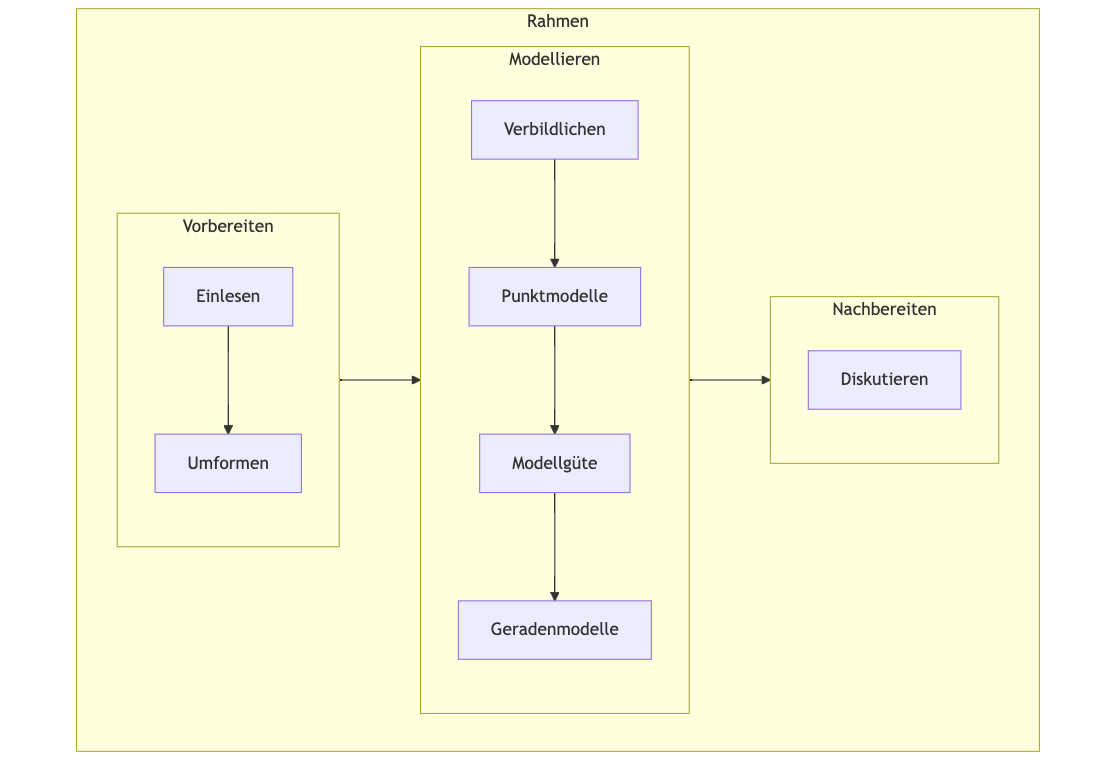
\includegraphics{img/fig-ueberblick.png}

}

\caption{\label{fig-ueberblick}Überblick über den Inhalt und Verlauf des
Buches}

\end{figure}%

Das Diagramm zeigt den Ablauf einer typischen Datenanalyse. Natürlich
kann man sich auch andere sinnvolle Darstellungen dieses Ablaufs
vorstellen.

\section{Software}\label{software}

Sie benötigen R, RStudio und einige R-Pakete für diesen Kurs.

\subsection{Installation}\label{installation}

\href{https://hinweisbuch.netlify.app/hinweise-software}{Hier} finden
Sie \emph{Installationshinweise.}\footnote{\url{https://hinweisbuch.netlify.app/hinweise-software}}

\subsection{Viel R (?)}\label{viel-r}

Dieses Buch enthält ``mittel'' viel R. Auf fortgeschrittene R-Techniken
wurde aber komplett verzichtet. Dem einen oder der anderen Anfänger:in
mag es dennoch ``viel Code'' erscheinen. Es wäre ja auch möglich
gewesen, auf R zu verzichten und stattdessen eine ``Klick-Software'' zu
verwenden. \href{https://jasp-stats.org/}{JASP} oder
\href{https://www.jamovi.org/}{Jamovi} sind Beispiele für tolle Software
aus dieser Kategorie. Ich glaube aber, der Verzicht auf eine
Skriptsprache (R) wäre ein schlechter Dienst an den Studentis. Mit Blick
auf eine ``High-Tech-Zukunft'' sollte man zumindest mit etwas
Computer-Code vertraut sein. Auf Computercode zu verzichten erschiene
mir daher fahrlässig für die ``Zukunftsfestigkeit'' der Ausbildung.

\section{Zum Autor}\label{zum-autor}

Nähere Hinweise zum Autor dieses Buch, Sebastian Sauer, finden Sie
\href{https://sebastiansauer-academic.netlify.app/}{hier}.\footnote{\url{https://sebastiansauer-academic.netlify.app/}}
Dort gibt es auch einen Überblick über
\href{https://sebastiansauer-academic.netlify.app/\#ebooks}{weitere
Bücher des Autors zum Themenkreis Datenanalyse}.\footnote{\url{https://sebastiansauer-academic.netlify.app/\#ebooks}}

\section{Nomenklatur}\label{nomenklatur}

\subsection{Griechische Buchstaben}\label{sec-greek}

In diesem Buch werden ein paar (wenige) griechische Buchstaben
verwendet, die in der Statistik üblich sind. Häufig werden
\emph{griechische} Buchstaben verwendet, um eine Grundgesamtheit
(Population) zu beschreiben (die meistens unbekannt ist). Lateinische
(``normale'') Buchstaben werden demgegenüber verwendet, um eine
Stichprobe (Datensatz, vorliegende Daten) zu beschreiben.
Tabelle~\ref{tbl-griech} stellt diese Buchstaben zusammen mit ihrer
Aussprache und Bedeutung vor.

\begin{longtable}[]{@{}lllr@{}}
\caption{Griechische Buchstaben, die in diesem Buch verwendet
werden.}\label{tbl-griech}\tabularnewline
\toprule\noalign{}
Zeichen & Aussprache & Buchstabe & Bedeutung in der Statistik \\
\midrule\noalign{}
\endfirsthead
\toprule\noalign{}
Zeichen & Aussprache & Buchstabe & Bedeutung in der Statistik \\
\midrule\noalign{}
\endhead
\bottomrule\noalign{}
\endlastfoot
\(\beta\) & beta & b & Regressionskoeffizent \\
\(\mu\) & mü & m & Mittelwert \\
\(\sigma\) & sigma & s & Streuung \\
\(\Sigma\) & Sigma & S & Summenzeichen \\
\(\rho\) & rho & r & Korrelation (nach Pearson) \\
\end{longtable}

Mehr griechische Buchstaben finden sich
\href{https://de.wikipedia.org/wiki/Griechisches_Alphabet}{z.B. in
Wikipedia}.\footnote{\url{https://de.wikipedia.org/wiki/Griechisches_Alphabet}}

\section{Zitation}\label{zitation}

Bitte zitieren Sie dieses Buch wie folgt:

\begin{quote}
Sauer, S. (2024). \emph{Statistik1}. https://statistik1.netlify.app/
\end{quote}

Hier sind die maschinenlesbaren Zitationsinfos (Bibtex-Format), die Sie
in Ihre Literatursoftware importieren können:

\begin{verbatim}
@book{sauer_statistik1,
    title = {Statistik1},
    rights = {CC-BY-NC},
    url = {https://statistik1.netlify.app/},
    author = {Sauer, Sebastian},
    date = {2024},
}
\end{verbatim}

Hier ist die DOI:

\href{https://zenodo.org/doi/10.5281/zenodo.10082517}{10.5281/zenodo.10082517}

\section{Reproduzierbarkeit}\label{reproduzierbarkeit}

Die verwendeten R-Pakete sind mit
\href{https://rstudio.github.io/renv/index.html}{renv}
dokumentiert.\footnote{\url{https://rstudio.github.io/renv/index.html}}

Der Quellcode ist \href{https://github.com/sebastiansauer/statistik1}{in
diesem Github-Repo} dokumentiert.\footnote{\url{https://github.com/sebastiansauer/statistik1}}

Dieses Dokument wurde erzeugt am/um: 2024-08-29 09:33:27.

\part{Organisatorisches}

\part{Modellieren}

\chapter{Modellgüte}\label{modellguxfcte}

\section{Lernsteuerung}\label{lernsteuerung}

\subsection{Standort im Lernpfad}\label{standort-im-lernpfad}

Abbildung~\ref{fig-ueberblick} zeigt den Standort dieses Kapitels im
Lernpfad und gibt damit einen Überblick über das Thema dieses Kapitels
im Kontext aller Kapitel.

\subsection{Lernziele}\label{lernziele-1}

\begin{itemize}
\tightlist
\item
  Sie kennen gängige Maße der Streuung einer Stichprobe und können diese
  definieren und mit Beispielen erläutern.
\item
  Sie können gängige Maße der Streuung einer Stichprobe mit R berechnen.
\item
  Sie können die Bedeutung von Streuung für die Güte eines Modells
  erläutern.
\end{itemize}

\subsection{Benötigte R-Pakete}\label{benuxf6tigte-r-pakete}

In diesem Kapitel benötigen Sie folgende R-Pakete.

\begin{Shaded}
\begin{Highlighting}[]
\FunctionTok{library}\NormalTok{(tidyverse)}
\FunctionTok{library}\NormalTok{(easystats)}
\FunctionTok{library}\NormalTok{(DataExplorer)}
\end{Highlighting}
\end{Shaded}

\subsection{Benötigte Daten}\label{benuxf6tigte-daten}

\begin{Shaded}
\begin{Highlighting}[]
\NormalTok{mariokart\_path }\OtherTok{\textless{}{-}} \FunctionTok{paste0}\NormalTok{(}
  \StringTok{"https://vincentarelbundock.github.io/Rdatasets/"}\NormalTok{,}
  \StringTok{"csv/openintro/mariokart.csv"}\NormalTok{)}

\NormalTok{mariokart }\OtherTok{\textless{}{-}} \FunctionTok{read.csv}\NormalTok{(mariokart\_path)}
\end{Highlighting}
\end{Shaded}

\subsection{Zum Einstieg}\label{zum-einstieg}

\begin{exercise}[Freiwillige
vor!]\protect\hypertarget{exr-streuung-erkennen}{}\label{exr-streuung-erkennen}

Für diese kleine Live-Demonstration brauchen wir einige Freiwillige. Die
Lehrkraft teilt die Freiwilligen in zwei Gruppen, Gruppe
\emph{Gleich-Groß} und Gruppe \emph{Verschieden-Groß}. Erkennen Sie,
dass die \emph{Unterschiedlichkeit} der Größe in Gruppe
\emph{Gleich-Groß} gering ist, aber in Gruppe \emph{Verschieden-Groß}
hoch? \(\square\)

\end{exercise}

\section{Warum Sie die Streuung Ihrer Daten kennen
sollten}\label{warum-sie-die-streuung-ihrer-daten-kennen-sollten}

\subsection{Die Schlankheitspille von
Prof.~Weiss-Ois}\label{sec-weiss-ois}

Prof.~Weiss-Ois hat eine Erfindung gemacht, eine Schlankheitspille
\ldots{}

\subsubsection{Was er sagt}\label{was-er-sagt}

\begin{figure}[H]

{\centering 
\includegraphics[width=0.25\textwidth,height=\textheight]{img/teacher.png}

}

\caption{``Ich habe eine Schlankheitspille entwickelt, die pro Einnahme
das Gewicht im Schnitt um 1kg reduziert!''}

\end{figure}%

\subsubsection{Was er NICHT sagt}\label{was-er-nicht-sagt}

\begin{figure}[H]

{\centering 
\includegraphics[width=0.25\textwidth,height=\textheight]{img/teacher.png}

}

\caption{``Allerdings streuten die Werte der Gewichtsveränderung um 10kg
um den Mittelwert herum.''}

\end{figure}%

\href{https://www.flaticon.com/free-icons/professor}{Icon unter Flaticon
licence, Autor: iconixar}

Würden Sie die Pille von Prof.~I. Ch. Weiss-Ois nehmen?\footnote{Ich auf
  keinen Fall.}

\begin{enumerate}
\def\labelenumi{\alph{enumi})}
\tightlist
\item
  ja
\item
  nein
\item
  Nur wenn ich 100 Euro bekomme
\item
  Okay, für 1000 Euro\(\square\)
\end{enumerate}

\begin{tcolorbox}[enhanced jigsaw, opacityback=0, arc=.35mm, left=2mm, colframe=quarto-callout-important-color-frame, toptitle=1mm, colback=white, toprule=.15mm, bottomrule=.15mm, colbacktitle=quarto-callout-important-color!10!white, bottomtitle=1mm, coltitle=black, titlerule=0mm, title=\textcolor{quarto-callout-important-color}{\faExclamation}\hspace{0.5em}{Wichtig}, rightrule=.15mm, breakable, leftrule=.75mm, opacitybacktitle=0.6]

Wie sehr die Werte eines Modells streuen, ist eine wichtige
Information.\(\square\)

\end{tcolorbox}

\subsection{Wie man seine Kuh über den Fluss
bringt}\label{wie-man-seine-kuh-uxfcber-den-fluss-bringt}

Treffen sich zwei Bauern, Fritz Furchenzieher und Karla Kartoffelsack.
Fritz will mit seiner Kuh einen Fluss überqueren, nur kann die Kuh nicht
schwimmen\footnote{ob es Fritz kann, ist nicht überliefert.}.

\begin{quote}
{\emoji{man-farmer}} (Fritz): Sag mal, Karla, ist der Fluss tief?
\end{quote}

\begin{quote}
{\emoji{woman-farmer}}(Karla): Nö, im Schnitt nur einen Meter.
\end{quote}

Also führt Fritz seine Kuh durch den Fluss, leider kam die Kuh nicht am
anderen Ufer an, im Floß ersoffen, s. Abbildung~\ref{fig-fluss-tief}.

\begin{figure}

\centering{

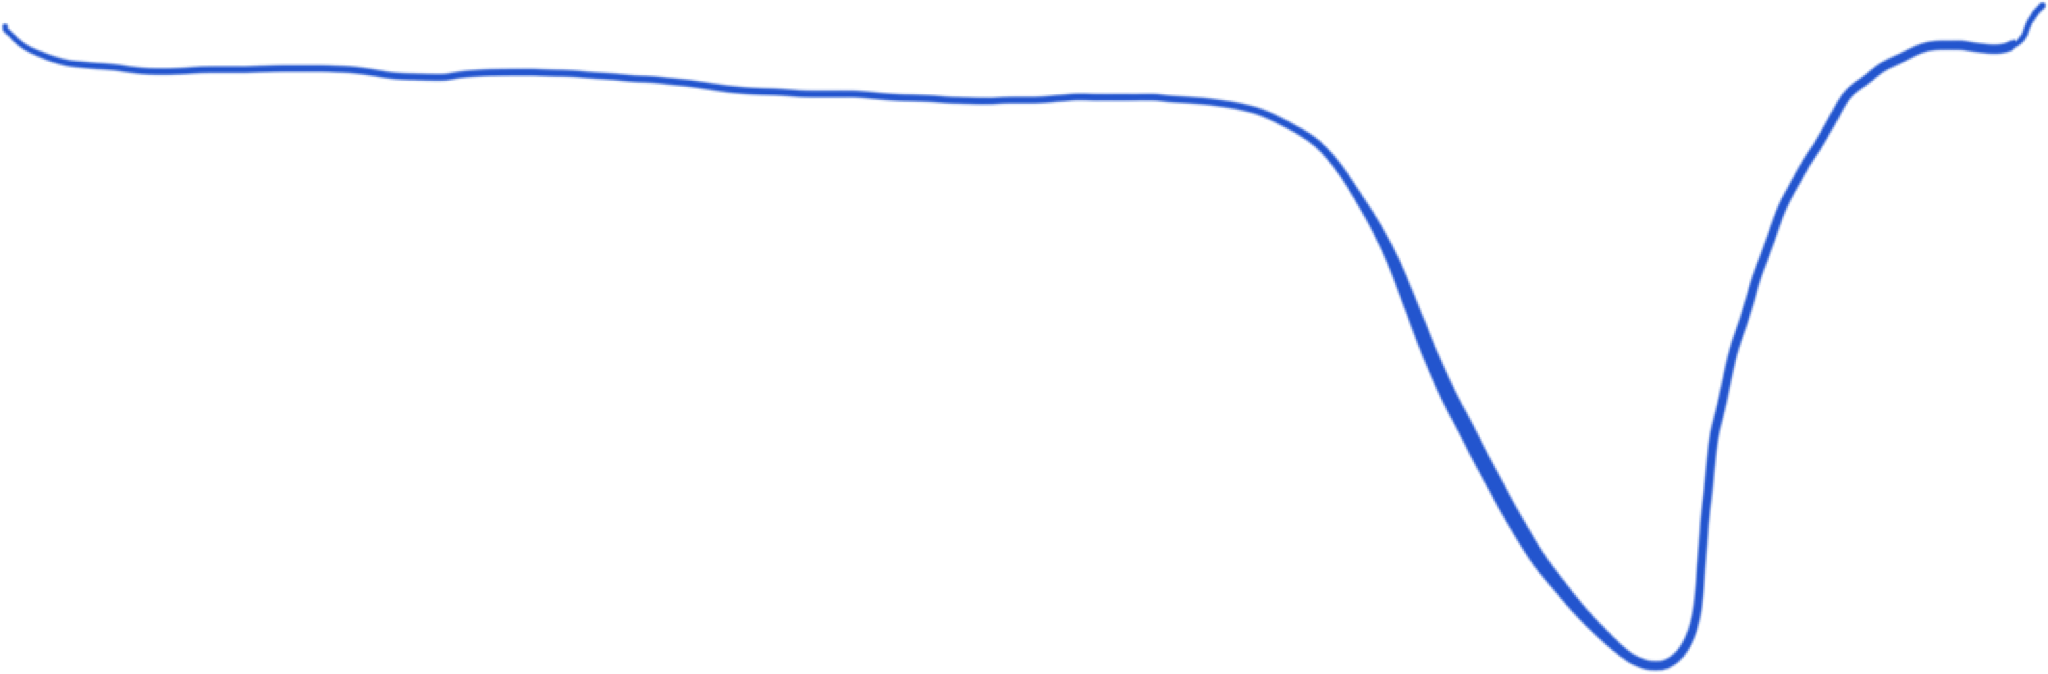
\includegraphics{img/fluss-tief.png}

}

\caption{\label{fig-fluss-tief}Der Fluss ist im Schnitt nur einen Meter
tief, trotzdem ist die Kuh ersoffen.}

\end{figure}%

\begin{quote}
{\emoji{woman-farmer}}(Karla): Übrigens, Lagemaße sagen nicht alles,
Fritz.
\end{quote}

\begin{quote}
{\emoji{man-farmer}}: Läuft die Kuh durch den Fluss, kann sie schwimmen
oder 's ist Schluss.
\end{quote}

\begin{tcolorbox}[enhanced jigsaw, opacityback=0, arc=.35mm, left=2mm, colframe=quarto-callout-important-color-frame, toptitle=1mm, colback=white, toprule=.15mm, bottomrule=.15mm, colbacktitle=quarto-callout-important-color!10!white, bottomtitle=1mm, coltitle=black, titlerule=0mm, title=\textcolor{quarto-callout-important-color}{\faExclamation}\hspace{0.5em}{Wichtig}, rightrule=.15mm, breakable, leftrule=.75mm, opacitybacktitle=0.6]

Die Streuung ihrer Daten zu kennen ist eine wesentliche Information.
\(\square\)

\end{tcolorbox}

\section{Woran erkennt man ein gutes
Modell?}\label{woran-erkennt-man-ein-gutes-modell}

Abbildung~\ref{fig-streuung} zeigt ein einfaches Modell (Mittelwert) mit
wenig Streuung (links) vs.~ein einfaches Modell mit viel Streuung
(rechts). Links ist die Streuung der Schlankheitspille
\emph{Dicktableitin} und rechts von der Schlankheitspille
\emph{Pfundafliptan} abgetragen.

\begin{figure}

\centering{

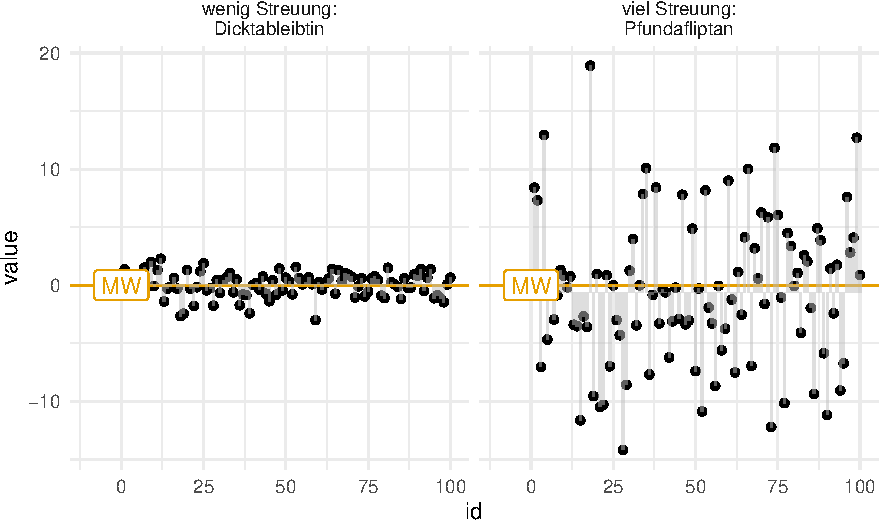
\includegraphics{060-modellguete_files/figure-pdf/fig-streuung-1.pdf}

}

\caption{\label{fig-streuung}Ein Modell mit wenig Streuung (links)
vs.~ein Modell mit viel Streuung (rechts). Die vertikalen grauen Balken
kennzeichnen den (absoluten) Abstand von jeweils einem Datenpunkt zum
Mittelwert (horizontale orange Linie). Je länger die `Abstandsbalken',
desto größer die Streuung.}

\end{figure}%

Bei einem Modell mit \emph{wenig} Streuung liegen die tatsächlichen,
beobachtete Werte (\(y\)) nah an den Modellwerten (vorhergesagten
Werten, \(\hat{y}\)); die Abweichungen \(e = y - \hat{y}\) sind also
gering (der Modellfehler ist klein). Bei einem Modell mit \emph{viel}
Streuung ist der Modellfehler \(e\) (im Vergleich dazu) groß.

\begin{example}[Daten zur Schlankheitskur von
Prof.~Weiss-Ois]\protect\hypertarget{exm-weiss-ois}{}\label{exm-weiss-ois}

In Abbildung~\ref{fig-streuung} sind die Daten zu der
Gewichtsveränderung nach Einnahme von ``Schlankheitspillen'' zweier
verschiedener Präparate. Wie man sieht unterscheidet sich die typische
(vorhergesagte) Gewichtsveränderung zwischen den beiden Präparaten kaum.
Die Streuung allerdings schon. Links sieht man die Gewichtsveränderungen
nach Einnahme des Präparats ``Dickableibtin extra mild'' (c) und rechts
das Präparat von Prof.~Weiss-Ois ``Pfundafliptan Forte''. Welches
Präparat würden Sie lieber einnehmen?\(\square\)

\end{example}

\begin{tcolorbox}[enhanced jigsaw, opacityback=0, arc=.35mm, left=2mm, colframe=quarto-callout-important-color-frame, toptitle=1mm, colback=white, toprule=.15mm, bottomrule=.15mm, colbacktitle=quarto-callout-important-color!10!white, bottomtitle=1mm, coltitle=black, titlerule=0mm, title=\textcolor{quarto-callout-important-color}{\faExclamation}\hspace{0.5em}{Wichtig}, rightrule=.15mm, breakable, leftrule=.75mm, opacitybacktitle=0.6]

Wir wollen ein präzises Modell, also kurze Fehlerbalken: Das Modell soll
die Daten gut erklären, also wenig vom tatsächlichen Wert abweichen.
Jedes Modell sollte Informationen über die Präzision des Modellwerts
bzw. der Modellwerte (Vorhersagen) angeben. Ein Modell ohne Angaben der
Modellgüte, d.h. der Präzision der Schätzung des Modellwerts, ist wenig
nütze.\(\square\)

\end{tcolorbox}

\begin{quote}
{\emoji{student}} Ich frage mich, ob man so ein Modell nicht verbessern
kann?
\end{quote}

\begin{quote}
{\emoji{teacher}} Die Frage ist, was wir mit ``verbessern'' meinen?
\end{quote}

\begin{quote}
{\emoji{student}} Naja, kürzere Fehlerbalken, ist doch klar!
\end{quote}

Da die Anzahl der Lenkräder mit dem Verkaufsgebot zusammenhängt, könnte
es vielleicht sein, dass wir die Lenkräder-Anzahl da irgendwie nutzen
könnten. Das sollten wir ausprobieren.

Abbildung~\ref{fig-fehler-red} zeigt, dass die Fehlerbalken
\emph{kürzer} werden, wenn wir ein (sinnvolles) komplexeres Modell
finden. Innerhalb jeder der beiden Gruppen (mit 2 Lenkrädern vs.~mit 0
Lenkrädern) sind die Fehlerbalken jeweils im Durchschnitt kürzer
(rechtes Teildiagramm) als im Modell ohne Gruppierung (linkes
Teildiagramm).\footnote{Aus Gründen der Übersichtlichkeit wurden nur
  Autos mit Verkaufsgebot von weniger als 100 Euros berücksichtigt und
  nur Spiele mit 0 oder mit 2 Lenkrädern.}

\begin{figure}

\begin{minipage}{0.50\linewidth}

\centering{

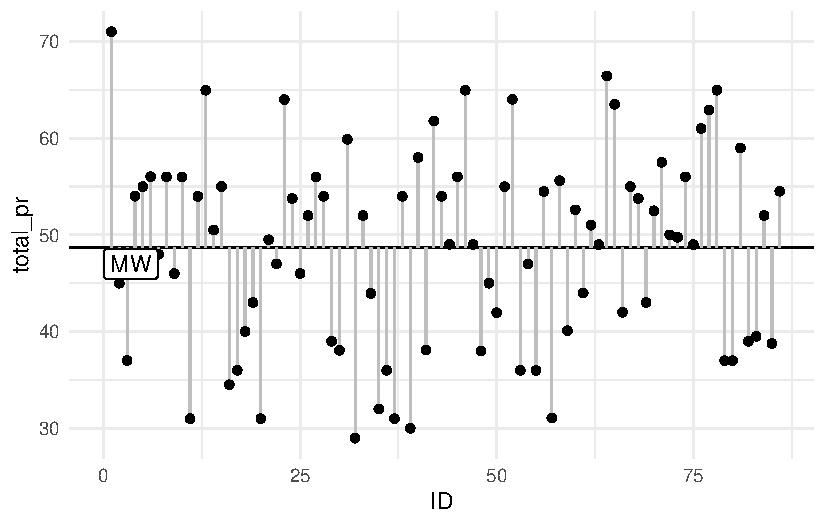
\includegraphics{060-modellguete_files/figure-pdf/fig-fehler-red-1.pdf}

}

\subcaption{\label{fig-fehler-red-1}Fehlerbalken im einfachen Modell:
Ein Mittelwert; viel Streuung insgesamt}

\end{minipage}%
%
\begin{minipage}{0.50\linewidth}

\centering{

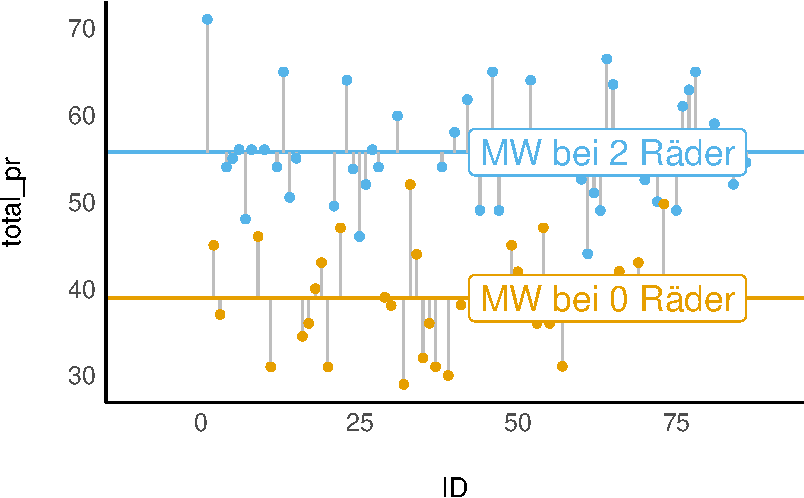
\includegraphics{060-modellguete_files/figure-pdf/fig-fehler-red-2.pdf}

}

\subcaption{\label{fig-fehler-red-2}Fehlerbalken im komplexen Modell:
Zwei Mittelwerte; weniger Streuung in jeder Gruppe. Das erkennt man
daran, dass die vertikalen, grauen Abstandsbalken im Schnitt kürzer sind
als im einfachen Modell (links)}

\end{minipage}%

\caption{\label{fig-fehler-red}Fehlerbalken in einem einfachen und
komplexeren Modell}

\end{figure}%

\begin{tcolorbox}[enhanced jigsaw, opacityback=0, arc=.35mm, left=2mm, colframe=quarto-callout-important-color-frame, toptitle=1mm, colback=white, toprule=.15mm, bottomrule=.15mm, colbacktitle=quarto-callout-important-color!10!white, bottomtitle=1mm, coltitle=black, titlerule=0mm, title=\textcolor{quarto-callout-important-color}{\faExclamation}\hspace{0.5em}{Wichtig}, rightrule=.15mm, breakable, leftrule=.75mm, opacitybacktitle=0.6]

Durch sinnvolle, komplexere Modelle sinkt die Fehlerstreuung eines
Modells.\(\square\)

\end{tcolorbox}

\section{Streuungsmaße}\label{sec-streuung}

\begin{definition}[Streuungsmaße]\protect\hypertarget{def-streuungsmaße}{}\label{def-streuungsmaße}

Ein Streuungsmaß quantifiziert die Variabilität eines Merkmals.
\(\square\)

\end{definition}

Ein einfaches Streuungsmaß ist der \emph{Range}, definiert als Abstand
von größtem und kleinsten Wert eines Merkmals. Dieses Mermals ist aber
nicht robust (gegenüber Extremwerten) und sollte daher nur mit
Einschränkung verwendet werden.

\subsection{Der mittlere
Abweichungsbalken}\label{der-mittlere-abweichungsbalken}

\begin{quote}
{\emoji{student}} Wir müssen jetzt mal präziser werden! Wie können wir
die Streuung berechnen?
\end{quote}

\begin{quote}
{\emoji{teacher}} Gute Frage! Am einfachsten ist es, wenn wir die
mittlere Länge eines Abweichungsbalkens ausrechnen.
\end{quote}

Legen wir (gedanklich) alle Abweichungsbalken \(e\) aneinander und
teilen durch die Anzahl \(n\) der Balken, so erhalten wir wir den
``mittleren Abweichungsbalken'', den wir mit \(\varnothing e\)
bezeichnen könnten. Diesen Kennwert bezeichnet man als \emph{Mean
Absolute Error} (MAE) bzw. als \emph{Mittlere Absolutabweichung} (MAA).
Er ist so definiert, s. Gleichung~\ref{eq-mae}.

\begin{equation}\phantomsection\label{eq-mae}{{\displaystyle \mathrm {MAE} ={\frac {\sum _{i=1}^{n}\left|y_{i}-\bar{y}\right|}{n}}={\frac {\sum _{i=1}^{n}\left|e_{i}\right|}{n}}.}}\end{equation}

\begin{definition}[Mittlere
Absolutabweichung]\protect\hypertarget{def-mae}{}\label{def-mae}

Die Mittlere Absolutabweichung (MAA, MAE) ist definiert als die Summe
der Absolutwerte der Differenzen eines Messwerts zum Mittelwert, geteilt
durch die Anzahl der Messwerte.\footnote{Wenn man solche Sätze liest,
  fühlt sich die Formel fast einfacher an.}\(\square\)

\end{definition}

\begin{example}[]\protect\hypertarget{exm-mae}{}\label{exm-mae}

Abbildung~\ref{fig-mae} visualisiert ein einfaches Beispiel zum MAE.
Rechnen wir den MAE für das Beispiel von Abbildung~\ref{fig-mae} aus:

\(MAE = \frac{1 + |- 3| + 1 + 1}{4} = 6/4 = 1.5\)

\end{example}

\begin{figure}

\centering{

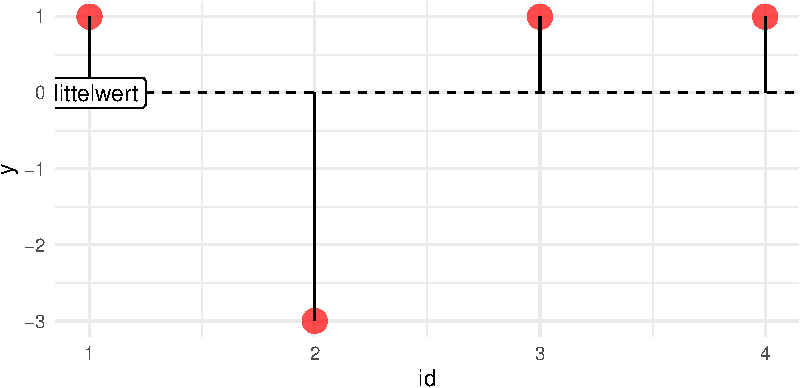
\includegraphics{060-modellguete_files/figure-pdf/fig-mae-1.pdf}

}

\caption{\label{fig-mae}Abweichungsbalken und der MAE}

\end{figure}%

Natürlich können wir R auch die Rechenarbeit überlassen.

\begin{quote}
{\emoji{robot}} Loving it!!
\end{quote}

Schauen Sie: Den Mittelwert (s. Abbildung~\ref{fig-mae}) kann man doch
mit Fug und Recht als ein \emph{lineares Modell}, eine Gerade,
betrachten, oder nicht? Schließlich erklären wir \(y\) anhand einer
Gerade (die parallel zur X-Achse ist).

In R gibt es einen Befehl für ein \emph{l}ineares \emph{M}odell, er
heißt \texttt{lm}.

Die Syntax von \texttt{lm()} lautet:

\texttt{lm(y\ \textasciitilde{}\ 1,\ data\ =\ meine\_daten)}.

In Worten:

\begin{quote}
Hey R, berechne mit ein lineares Modell zur Erklärung von Y. Aber
verwende keine andere Variable zur Erklärung von Y, sondern nimm den
Mittelwert von Y.
\end{quote}

\begin{Shaded}
\begin{Highlighting}[]
\NormalTok{lm1 }\OtherTok{\textless{}{-}} \FunctionTok{lm}\NormalTok{(y }\SpecialCharTok{\textasciitilde{}} \DecValTok{1}\NormalTok{, }\AttributeTok{data =}\NormalTok{ d)}
\end{Highlighting}
\end{Shaded}

Den MAE können wir uns jetzt so ausgeben lassen:

\begin{Shaded}
\begin{Highlighting}[]
\FunctionTok{mae}\NormalTok{(lm1)}
\DocumentationTok{\#\# [1] 1.5}
\end{Highlighting}
\end{Shaded}

\subsection{Der Interquartilsabstand}\label{der-interquartilsabstand}

Der Interquartilsabstand (IQA; engl. inter quartile range, IQR) ist ein
Streuungsmaß, das nicht auf dem Mittelwert aufbaut. Der IQR ist robuster
als z.B. der MAA oder die Varianz und die Standardabweichung.

\begin{definition}[Interquartilsabstand]\protect\hypertarget{def-iqr}{}\label{def-iqr}

Der Interquartilsabstand ist definiert als der die (absolute) Differenz
vom 3. Quartil und 1. Quartil.\(\square\)

\end{definition}

\begin{example}[IQR im
Hörsaal]\protect\hypertarget{exm-iqr}{}\label{exm-iqr}

In einem Statistikkurs betragen die Quartile der Körpergröße: Q1: 1.65m,
Q2 (Median): 1,70m, Q3: 1.75m. Der IQR beträgt dann:
\(IQR = Q3-Q1 = 1.75m - 1.65m = 0.10m\), d.h. 10 cm.\(\square\)

\end{example}

Abbildung~\ref{fig-iqr-mario} stellt den IQR (und einige Quantile) für
den Verkaufspreise von Mariokart-Spielen dar.

\begin{figure}

\centering{

\subsection{Histogramm}

\centering{

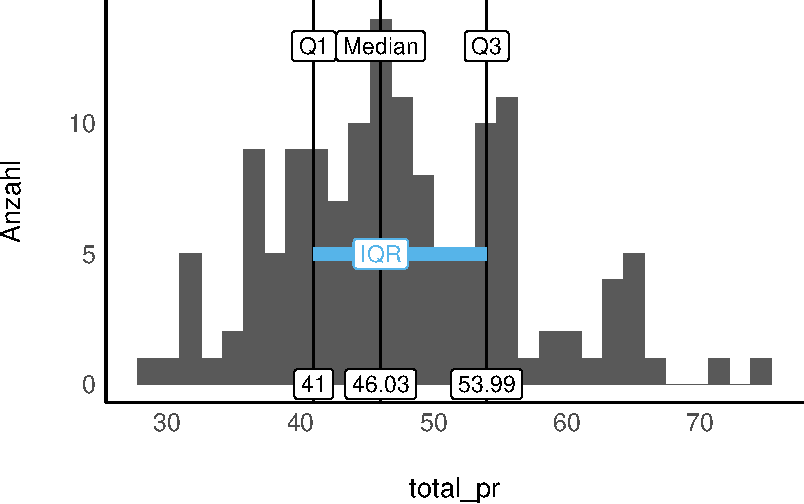
\includegraphics{060-modellguete_files/figure-pdf/fig-mario-qs-iqr1-1.pdf}

}

\subcaption{\label{fig-mario-qs-iqr1}IQR, Q1, Q2 und Q3 für das
Schlussgebot (nur Spiele für weniger als 100 Euro)}

\subsection{Dichtediagramm}

\centering{

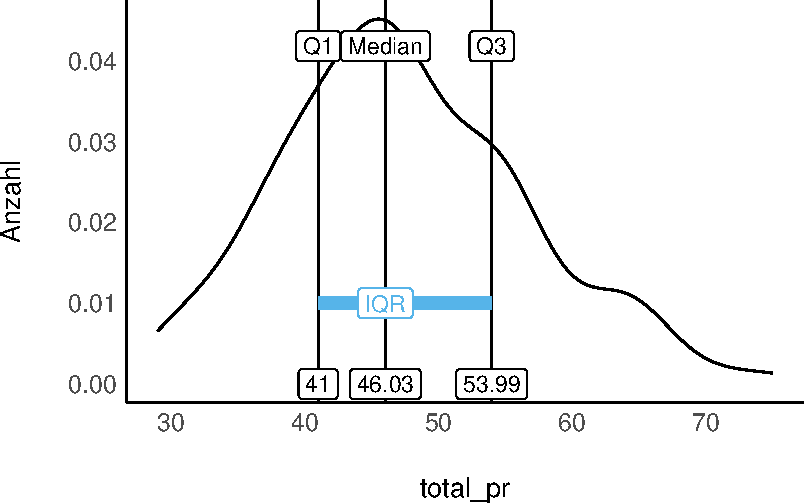
\includegraphics{060-modellguete_files/figure-pdf/fig-mario-iqr2-1.pdf}

}

\subcaption{\label{fig-mario-iqr2}IQR, Q1, Q2 und Q3 für das
Schlussgebot (nur Spiele für weniger als 100 Euro)}

}

\caption{\label{fig-iqr-mario}Der IQR für den Verkaufspreis von
Mariokart-Spielen.}

\end{figure}%

\subsection{Streuungsmaße für
Normalverteilungen}\label{streuungsmauxdfe-fuxfcr-normalverteilungen}

Normalverteilungen sind recht häufig anzutreffen in der Praxis der
Datenanalyse. Daher lohnt es sich, zu überlegen, wie man diese
Verteilungen gut zusammenfasst. Man kann zeigen, dass eine
Normalverteilung sich komplett über ihren \emph{Mittelwert} sowie ihre
\emph{Standardabweichung} beschreiben lässt. Außerdem gilt: Sind Ihre
Daten normalverteilt, dann sind die Abweichungen vom Mittelwert auch
normalverteilt. Denn wenn man eine Konstante zu einer Verteilung addiert
(bzw. subtrahiert), ``verschiebt man den Berg'' ja nur zur Seite, ohne
seine Form zu verändern, s. Abbildung~\ref{fig-norm-dev}.

\begin{tcolorbox}[enhanced jigsaw, opacityback=0, arc=.35mm, left=2mm, colframe=quarto-callout-note-color-frame, toptitle=1mm, colback=white, toprule=.15mm, bottomrule=.15mm, colbacktitle=quarto-callout-note-color!10!white, bottomtitle=1mm, coltitle=black, titlerule=0mm, title=\textcolor{quarto-callout-note-color}{\faInfo}\hspace{0.5em}{Hinweis}, rightrule=.15mm, breakable, leftrule=.75mm, opacitybacktitle=0.6]

Hat man normalverteilte Variablen/Abweichungen/Residuen, so ist die
\emph{Standardabweichung} (engl. standard deviation, SD, \(\sigma\),
\(s\)) eine komfortable Maßeinheit der Streuung, denn damit lässt sich
die Streuung (Abweichung vom Mittelwert, Residuen) der Normalverteilung
gut beschreiben.\(\square\)

\end{tcolorbox}

\begin{quote}
{\emoji{student}} Aber wie berechnet man jetzt diese Standardabweichung?
\end{quote}

\begin{quote}
{\emoji{teacher}} Moment, noch ein kurzer Exkurs zur Varianz \ldots{}
\end{quote}

\begin{quote}
{\emoji{student}} (seufzt)
\end{quote}

\subsection{Varianz}\label{varianz}

\subsubsection{Intuition}\label{intuition}

\begin{tcolorbox}[enhanced jigsaw, opacityback=0, arc=.35mm, left=2mm, colframe=quarto-callout-note-color-frame, toptitle=1mm, colback=white, toprule=.15mm, bottomrule=.15mm, colbacktitle=quarto-callout-note-color!10!white, bottomtitle=1mm, coltitle=black, titlerule=0mm, title=\textcolor{quarto-callout-note-color}{\faInfo}\hspace{0.5em}{Hinweis}, rightrule=.15mm, breakable, leftrule=.75mm, opacitybacktitle=0.6]

Die Varianz einer Variable (z.B. Verkaufspreis von Mariokart) ist, grob
gesagt, der typische Abstand eines Verkaufspreis vom mittleren
Verkaufspreis.\(\square\)

\end{tcolorbox}

Abbildung~\ref{fig-var} illustriert die Varianz:

\begin{enumerate}
\def\labelenumi{\arabic{enumi}.}
\tightlist
\item
  Man gehe von der Häufigkeitsverteilung der Daten aus.
\item
  Betrachtet man die Daten als Gewichte auf einer Wippe, so ist der
  Schwerpunkt der Wippe der Mittelwert.
\item
  Man bilde Quadrate für jeden Datenpunkt mit der Kantenlänge, die dem
  Abstand des Punktes zum Mittelwert entspricht.
\item
  Die Quadrate quetscht man jetzt wo nötig in rechteckige Formen (ohne
  dass sich die Fläche ändern darf) und verschiebt sie, bis sich alle
  Formen zu einem Rechteck mit Seitenlänge \(n\) und \(\sigma^2\)
  anordnen.
\end{enumerate}

\begin{figure}

\centering{

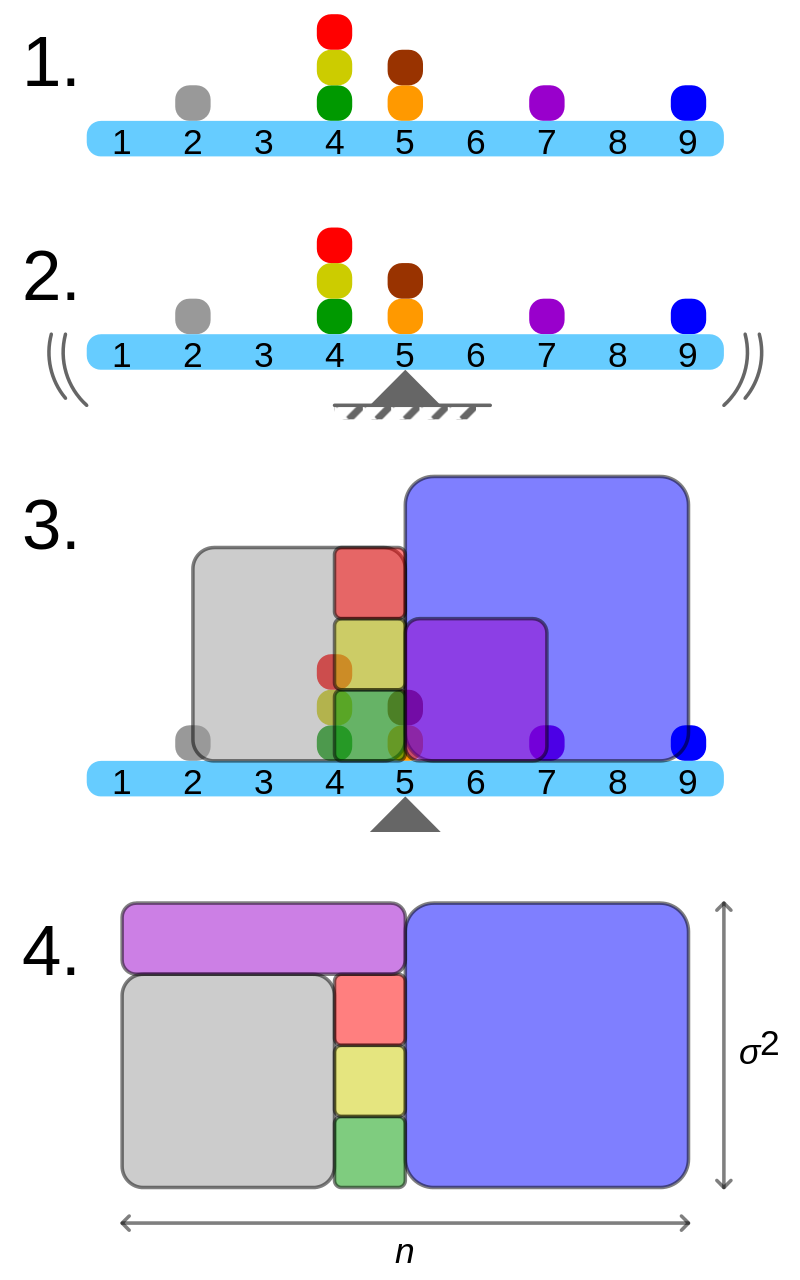
\includegraphics{img/Variance_visualisation.svg.png}

}

\caption{\label{fig-var}Illustration zur Varianz als ``mittlerer
Quadratfehler''}

\end{figure}%

\href{https://commons.wikimedia.org/w/index.php?curid=39472834}{By
Cmglee - Own work, CC BY-SA 3.0}

Abbildung~\ref{fig-mse} visualisiert die Varianz für
Beispiel~\ref{exm-mae}.\footnote{Die Abweichungsquadrate wirken optisch
  nicht quadratisch, da die X-Achse breiter skaliert dargestellt ist als
  die Y-Achse. Trotzdem sind es Quadrate, nur nicht optisch, wenn Sie
  wissen, was ich meine\ldots{}}

Links sind die \emph{Abweichungsquadrate} dargestellt, rechts die
Varianz als ``\emph{typisches Abweichungsquadrat}''.

\begin{tcolorbox}[enhanced jigsaw, opacityback=0, arc=.35mm, left=2mm, colframe=quarto-callout-note-color-frame, toptitle=1mm, colback=white, toprule=.15mm, bottomrule=.15mm, colbacktitle=quarto-callout-note-color!10!white, bottomtitle=1mm, coltitle=black, titlerule=0mm, title=\textcolor{quarto-callout-note-color}{\faInfo}\hspace{0.5em}{Hinweis}, rightrule=.15mm, breakable, leftrule=.75mm, opacitybacktitle=0.6]

Die Varianz ist also ein Maß, das die typische Abweichung der
Beobachtungen vom Mittelwert in eine Zahl fasst.\(\square\)

\end{tcolorbox}

\begin{figure}

\begin{minipage}{0.50\linewidth}

\centering{

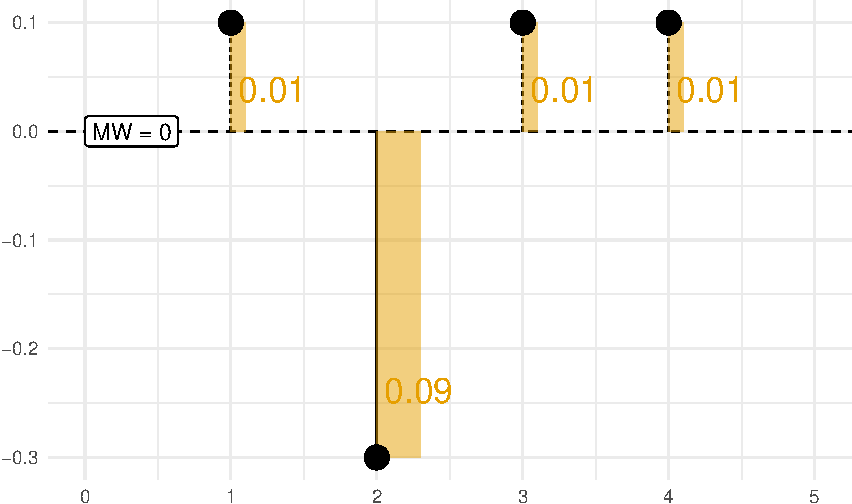
\includegraphics{060-modellguete_files/figure-pdf/fig-mse-1.pdf}

}

\subcaption{\label{fig-mse-1}Quadrierte Fehlerbalken}

\end{minipage}%
%
\begin{minipage}{0.50\linewidth}

\centering{

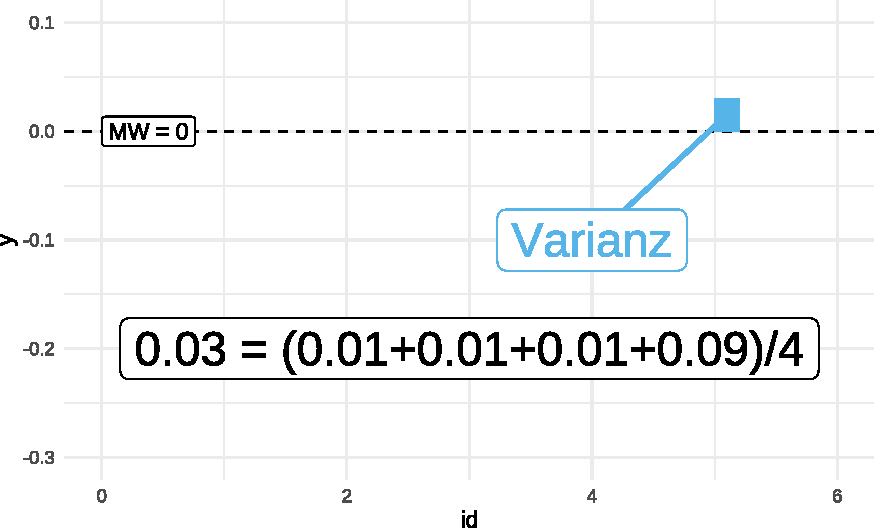
\includegraphics{060-modellguete_files/figure-pdf/fig-mse-2.pdf}

}

\subcaption{\label{fig-mse-2}Varianz als `typischer' Fehlerbalken}

\end{minipage}%

\caption{\label{fig-mse}Sinnbild zur Varianz als typischer Fehlerbalken}

\end{figure}%

\begin{example}[]\protect\hypertarget{exm-var}{}\label{exm-var}

Sie arbeiten immer noch bei einem Online-Auktionshaus und untersuchen
den Verkauf von Videospielen. Natürlich mit dem Ziel, dass Ihre Firma
mehr von dem Zeug verkaufen kann.

Dazu berechnen Sie die Streuung in den Verkaufspreisen, s.
Listing~\ref{lst-mario-streu}. \(\square\)

\end{example}

\begin{codelisting}

\caption{\label{lst-mario-streu}Berechnung der Streuung des
Verkaufpreises als Indikatoren für die Modellgüte des Mittelwerts.}

\centering{

\begin{Shaded}
\begin{Highlighting}[]
\NormalTok{mariokart\_no\_extreme }\OtherTok{\textless{}{-}}
\NormalTok{  mariokart }\SpecialCharTok{\%\textgreater{}\%}
  \FunctionTok{filter}\NormalTok{(total\_pr }\SpecialCharTok{\textless{}} \DecValTok{100}\NormalTok{)  }\CommentTok{\# ohne Extremwerte}

\NormalTok{m\_summ }\OtherTok{\textless{}{-}} 
\NormalTok{  mariokart\_no\_extreme }\SpecialCharTok{\%\textgreater{}\%} 
  \FunctionTok{summarise}\NormalTok{(}
    \AttributeTok{pr\_mw =} \FunctionTok{mean}\NormalTok{(total\_pr),}
    \AttributeTok{pr\_iqr =} \FunctionTok{IQR}\NormalTok{(total\_pr),}
    \AttributeTok{pr\_maa =} \FunctionTok{mean}\NormalTok{(}\FunctionTok{abs}\NormalTok{(total\_pr }\SpecialCharTok{{-}} \FunctionTok{mean}\NormalTok{(total\_pr))),}
    \AttributeTok{pr\_var =} \FunctionTok{var}\NormalTok{(total\_pr),}
    \AttributeTok{pr\_sd =} \FunctionTok{sd}\NormalTok{(total\_pr))}
\end{Highlighting}
\end{Shaded}

}

\end{codelisting}%

\begin{longtable}[]{@{}lrrrr@{}}
\toprule\noalign{}
pr\_mw & pr\_iqr & pr\_maa & pr\_var & pr\_sd \\
\midrule\noalign{}
\endhead
\bottomrule\noalign{}
\endlastfoot
47.43 & 12.99 & 7.20 & 83.06 & 9.11 \\
\end{longtable}

Statistiken sind ja schön \ldots{} aber Bilder sind auch gut, s.
Abbildung~\ref{fig-var}. Datendiagramme eignen sich gut, um (grob) die
Streuung einer Variable zu erfassen.

\begin{Shaded}
\begin{Highlighting}[]
\NormalTok{mariokart }\SpecialCharTok{\%\textgreater{}\%} 
\NormalTok{  mariokart }\SpecialCharTok{\%\textgreater{}\%} 
  \FunctionTok{select}\NormalTok{(total\_pr) }\SpecialCharTok{\%\textgreater{}\%} 
  \FunctionTok{filter}\NormalTok{(total\_pr }\SpecialCharTok{\textless{}} \DecValTok{100}\NormalTok{) }\SpecialCharTok{\%\textgreater{}\%}  \CommentTok{\# ohne Extremwerte}
  \FunctionTok{plot\_density}\NormalTok{()}
\end{Highlighting}
\end{Shaded}

\begin{figure}

\begin{minipage}{0.50\linewidth}

\centering{

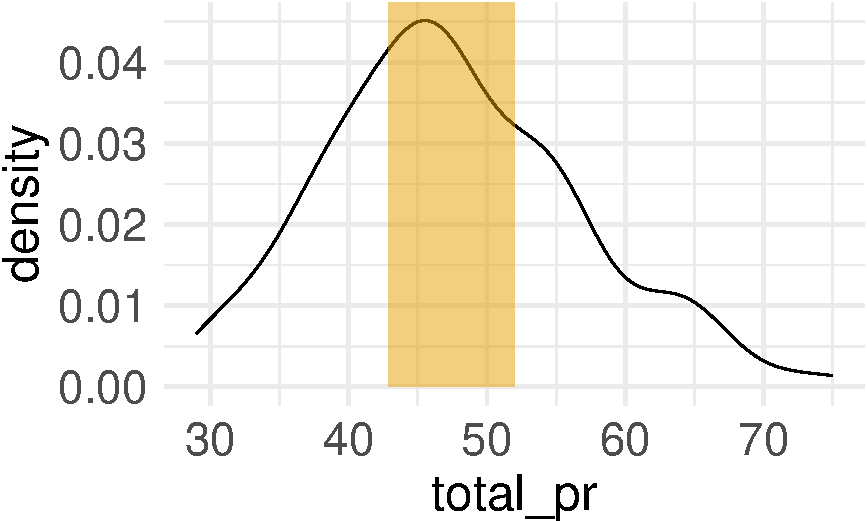
\includegraphics{060-modellguete_files/figure-pdf/fig-var-1.pdf}

}

\subcaption{\label{fig-var-1}Dichtediagramm mit MW±SD in roter Farbe}

\end{minipage}%
%
\begin{minipage}{0.50\linewidth}

\centering{

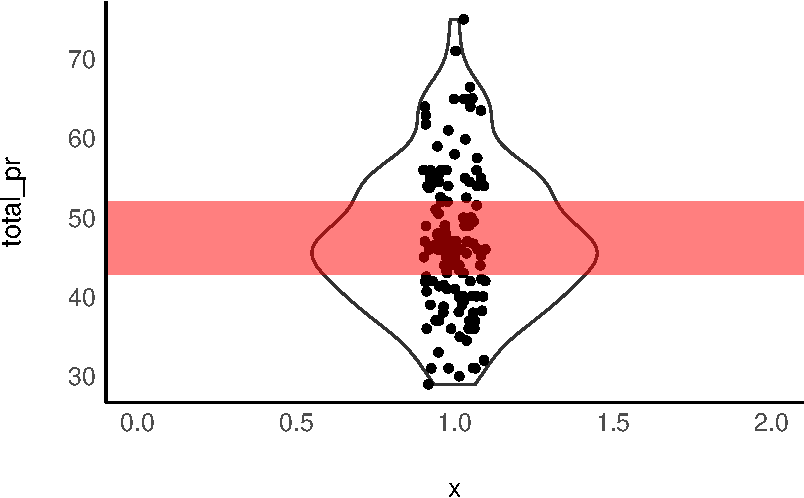
\includegraphics{060-modellguete_files/figure-pdf/fig-var-2.pdf}

}

\subcaption{\label{fig-var-2}Violindiagramm mit MW±SD in roter Farbe}

\end{minipage}%

\caption{\label{fig-var}Die Verteilung des Verkaufspreises von
Mariokart-Spielen}

\end{figure}%

Wer sich die Berechnung von Hand für \texttt{pr\_maa} sparen möchte (s.
Listing~\ref{lst-mario-streu}), kann die
\href{https://rdrr.io/cran/DescTools/man/MeanAD.html}{Funktion
\texttt{MeanAD} aus dem Paket \texttt{DescTools}} nutzen.

\subsubsection{Kochrezept für die
Varianz}\label{kochrezept-fuxfcr-die-varianz}

Um die Standardabweichung zu berechnen, berechnet man zunächst die
\emph{Varianz}, \(s^2\) abgekürzt. Hier ist ein
``Kochrezept''\footnote{Algorithmus} zur Berechnung der Varianz:

\begin{enumerate}
\def\labelenumi{\arabic{enumi}.}
\tightlist
\item
  Für alle Datenpunkte \(x_i\): Berechne die Abweichungen vom
  Mittelwert, \(\bar{x}\)
\item
  Quadriere diese Werte
\item
  Summiere dann auf
\item
  Teile durch die Anzahl \(N\) der Werte
\end{enumerate}

Als Formel ausgedrückt, lautet die Definition der Varianz\footnote{sog.
  unkorrigierte Stichprobenvarianz; um anhand einer Stichprobe die
  Varianz der zugehörigen Population zu schätzen, teilt man nicht durch
  \(N\), sondern durch \(N-1\)} einer Stichprobe wie folgt, s.
Gleichung~\ref{eq-var}.

\begin{equation}\phantomsection\label{eq-var}{{\displaystyle s^{2}={\frac {1}{N}}\sum _{i=1}^{n}\left(y_{i}-{\bar {y}}\right)^{2}={\frac {1}{N}}\sum _{i=1}^{n}e_i^{2}.}}\end{equation}

\begin{definition}[Varianz]\protect\hypertarget{def-var}{}\label{def-var}

Die Varianz (\(s^2, \sigma^2\)) ist definiert als der Mittelwert der
quadrierten Abweichungen, \(e_i^2\), (vom Mittelwert).\(\square\)

\end{definition}

Die Varianz steht im engen Verhältnis zur Kovarianz, s.
\textbf{?@sec-cov}. Die Varianz kann auch verstehen als den
\emph{mittleren Quadratfehler} (Mean Squared Error, MSE) eines Modells,
s. Gleichung~\ref{eq-mse}.

\begin{equation}\phantomsection\label{eq-mse}{{\displaystyle MSE={\frac {1}{N}}\sum _{i=1}^{N}\left(y_{i}-{\hat {y}}\right)^{2}.}}\end{equation}

Im Fall eines Punktmodells ist der Mittelwert der vorhergesagte Wert
eines Modells.

\subsection{Die Standardabweichung}\label{die-standardabweichung}

Kennt man die Varianz, so lässt sich die Standardabweichung einfach als
Quadratwurzel der Varianz berechnen.

\begin{definition}[Standardabweichung]\protect\hypertarget{def-sd}{}\label{def-sd}

Die Standardabweichung (SD, s, \(\sigma\)) ist definiert als die
Quadratwurzel der Varianz, s. Gleichung~\ref{eq-sd}.

\begin{equation}\phantomsection\label{eq-sd}{s := \sqrt{s^2} \square}\end{equation}

\end{definition}

Durch das Wurzelziehen besitzt die Standardabweichung wieder \emph{in
etwa} die gleiche Größenordnung wie die Daten (im Gegensatz zur Varianz,
die durch das Quadrieren sehr groß werden kann).

Aus einem Modellierungsblickwinkel kann man die SD definieren als die
Wurzel von MSE. Dann nennt man sie \emph{Root Mean Squared Error}
(RMSE): \(RMSE := \sqrt{MSE}\).

\begin{tcolorbox}[enhanced jigsaw, opacityback=0, arc=.35mm, left=2mm, colframe=quarto-callout-note-color-frame, toptitle=1mm, colback=white, toprule=.15mm, bottomrule=.15mm, colbacktitle=quarto-callout-note-color!10!white, bottomtitle=1mm, coltitle=black, titlerule=0mm, title=\textcolor{quarto-callout-note-color}{\faInfo}\hspace{0.5em}{Hinweis}, rightrule=.15mm, breakable, leftrule=.75mm, opacitybacktitle=0.6]

Die SD ist i.d.R. \emph{un}gleich zur MAE, aber (fast) gleich zur RMSE.
Entsprechend ist die Varianz (fast) gleich zur MSE.\(\square\)

\end{tcolorbox}

\begin{example}[]\protect\hypertarget{exm-sd-mario}{}\label{exm-sd-mario}

Sie arbeiten weiter an Ihrem Mariokart-Projekt. Da Sie heute keine Lust
auf viel Tippen haben, nutzen Sie das R-Paket \texttt{easystats} mit der
Funktion \texttt{describe\_distribution}.

\begin{Shaded}
\begin{Highlighting}[]
\FunctionTok{library}\NormalTok{(easystats)}

\NormalTok{mariokart }\SpecialCharTok{\%\textgreater{}\%} 
  \FunctionTok{select}\NormalTok{(total\_pr) }\SpecialCharTok{\%\textgreater{}\%} 
  \FunctionTok{describe\_distribution}\NormalTok{()}
\end{Highlighting}
\end{Shaded}

\begin{longtable}[]{@{}
  >{\raggedright\arraybackslash}p{(\columnwidth - 18\tabcolsep) * \real{0.1154}}
  >{\raggedleft\arraybackslash}p{(\columnwidth - 18\tabcolsep) * \real{0.1154}}
  >{\raggedleft\arraybackslash}p{(\columnwidth - 18\tabcolsep) * \real{0.1154}}
  >{\raggedleft\arraybackslash}p{(\columnwidth - 18\tabcolsep) * \real{0.0769}}
  >{\raggedleft\arraybackslash}p{(\columnwidth - 18\tabcolsep) * \real{0.0769}}
  >{\raggedleft\arraybackslash}p{(\columnwidth - 18\tabcolsep) * \real{0.0897}}
  >{\raggedleft\arraybackslash}p{(\columnwidth - 18\tabcolsep) * \real{0.1154}}
  >{\raggedleft\arraybackslash}p{(\columnwidth - 18\tabcolsep) * \real{0.1154}}
  >{\raggedleft\arraybackslash}p{(\columnwidth - 18\tabcolsep) * \real{0.0513}}
  >{\raggedleft\arraybackslash}p{(\columnwidth - 18\tabcolsep) * \real{0.1282}}@{}}
\toprule\noalign{}
\begin{minipage}[b]{\linewidth}\raggedright
Variable
\end{minipage} & \begin{minipage}[b]{\linewidth}\raggedleft
Mean
\end{minipage} & \begin{minipage}[b]{\linewidth}\raggedleft
SD
\end{minipage} & \begin{minipage}[b]{\linewidth}\raggedleft
IQR
\end{minipage} & \begin{minipage}[b]{\linewidth}\raggedleft
Min
\end{minipage} & \begin{minipage}[b]{\linewidth}\raggedleft
Max
\end{minipage} & \begin{minipage}[b]{\linewidth}\raggedleft
Skewness
\end{minipage} & \begin{minipage}[b]{\linewidth}\raggedleft
Kurtosis
\end{minipage} & \begin{minipage}[b]{\linewidth}\raggedleft
n
\end{minipage} & \begin{minipage}[b]{\linewidth}\raggedleft
n\_Missing
\end{minipage} \\
\midrule\noalign{}
\endhead
\bottomrule\noalign{}
\endlastfoot
total\_pr & 49.88049 & 25.68856 & 12.99 & 28.98 & 326.51 & 9.035897 &
96.14414 & 143 & 0 \\
\end{longtable}

Ah! Das war einfach. Wird auch langsam Zeit für Feierabend.\(\square\)

\end{example}

\begin{example}[]\protect\hypertarget{exm-gruppen-mw}{}\label{exm-gruppen-mw}

Ihr Job als Datenanalyst ist anstrengend, aber auch mitunter
interessant. So auch heute. Bevor Sie nach Hause gehen, möchten Sie noch
eine Sache anschauen. In einer früheren Analyse (s.
Abbildung~\ref{fig-fehler-red}) fanden Sie heraus, dass die Fehlerbalken
kürzer werden, wenn man ein geschickteres und komplexeres Modell findet.
Das wollen Sie natürlich prüfen. Sie überlegen: ``Okay, ich will ein
einfaches Modell, in dem der Mittelwert das Modell des Verkaufspreis
sein soll.''

Das spezifizieren Sie so:

\begin{Shaded}
\begin{Highlighting}[]
\NormalTok{lm1 }\OtherTok{\textless{}{-}} \FunctionTok{lm}\NormalTok{(total\_pr }\SpecialCharTok{\textasciitilde{}} \DecValTok{1}\NormalTok{, }\AttributeTok{data =}\NormalTok{ mariokart)}
\FunctionTok{mae}\NormalTok{(lm1)}
\DocumentationTok{\#\# [1] 10.01811}
\end{Highlighting}
\end{Shaded}

Im nächsten Schritt spezifizieren Sie ein Modell, in dem der
Verkaufpreis eine Funktion der Anzahl der Lenkräder ist (ähnlich wie in
Abbildung~\ref{fig-fehler-red}):

\begin{Shaded}
\begin{Highlighting}[]
\NormalTok{lm2 }\OtherTok{\textless{}{-}} \FunctionTok{lm}\NormalTok{(total\_pr }\SpecialCharTok{\textasciitilde{}}\NormalTok{ wheels, }\AttributeTok{data =}\NormalTok{ mariokart)}
\FunctionTok{mae}\NormalTok{(lm2)}
\DocumentationTok{\#\# [1] 7.375873}
\end{Highlighting}
\end{Shaded}

Ah! Sehr schön, Sie haben mit \texttt{lm2} ein besseres Modell als
einfach nur den Mittelwert gefunden. Ab nach hause!\(\square\)

\end{example}

\section{Streuung als Modellfehler}\label{streuung-als-modellfehler}

Wenn wir den Mittelwert als Punktmodell des Verkaufpreises auffassen, so
kann man die verschiedenen Kennwerte der Streuung als verschiedene
Kennwerte der Modellgüte auffassen.

Definieren wir zunächst als Punktmodell auf Errisch:

\begin{Shaded}
\begin{Highlighting}[]
\NormalTok{lm\_mario1 }\OtherTok{\textless{}{-}} \FunctionTok{lm}\NormalTok{(total\_pr }\SpecialCharTok{\textasciitilde{}} \DecValTok{1}\NormalTok{, }\AttributeTok{data =}\NormalTok{ mariokart)}
\end{Highlighting}
\end{Shaded}

Zur Erinnerung: Wir modellieren \texttt{total\_pr} ohne Prädiktoren,
sondern als Punktmodell, und zwar schätzen wir den Mittelwert mit den
Daten \texttt{mariokoart}.

Das (Meta-)Paket \texttt{easystats} bietet komfortable Befehle, um die
Modellgüte zu berechnen:

\begin{Shaded}
\begin{Highlighting}[]
\FunctionTok{mae}\NormalTok{(lm\_mario1)  }\CommentTok{\# Mean absolute error}
\DocumentationTok{\#\# [1] 10.01811}
\FunctionTok{mse}\NormalTok{(lm\_mario1)  }\CommentTok{\# Mean squared error}
\DocumentationTok{\#\# [1] 655.2874}
\FunctionTok{rmse}\NormalTok{(lm\_mario1)  }\CommentTok{\# Root mean squared error}
\DocumentationTok{\#\# [1] 25.59858}
\end{Highlighting}
\end{Shaded}

\section{z-Transformation}\label{z-transformation}

Sie arbeiten immer noch als Datenknecht, Moment, \emph{Datenhecht} bei
dem Online-Auktionshaus. Heute untersuchen Sie die Frage, wie gut sich
die Verkaufspreise mit einer einzeigen Zahl, dem mittleren
Verkaufspreis, beschreiben lassen. Einige widerspenstige Werte haben Sie
dabei einfach des Datensatzes verwiesen. Schon ist das Leben leichter,
s. \texttt{mariokart\_no\_extreme}.

\begin{Shaded}
\begin{Highlighting}[]
\NormalTok{mariokart\_no\_extreme }\OtherTok{\textless{}{-}} 
\NormalTok{  mariokart }\SpecialCharTok{\%\textgreater{}\%} 
  \FunctionTok{filter}\NormalTok{(total\_pr }\SpecialCharTok{\textless{}} \DecValTok{100}\NormalTok{)}
\end{Highlighting}
\end{Shaded}

Abbildung~\ref{fig-mariokart_no_extreme} (links) zeigt, dass es einige
Streuung um den Mittelwert herum gibt.
Abbildung~\ref{fig-mariokart_no_extreme} (rechts) zeigt die (um den
Mittelwert) \emph{zentrierten} Daten.

\begin{figure}

\begin{minipage}{0.50\linewidth}

\centering{

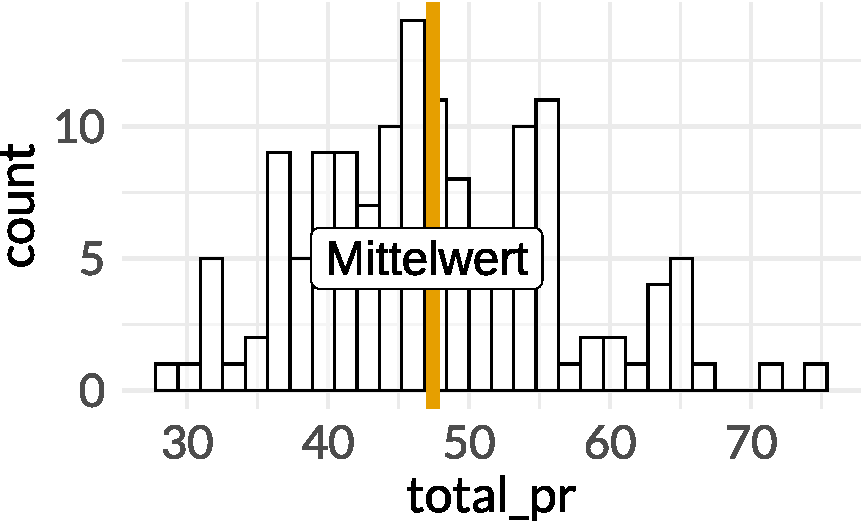
\includegraphics{060-modellguete_files/figure-pdf/fig-mariokart_no_extreme-1.pdf}

}

\subcaption{\label{fig-mariokart_no_extreme-1}Wie nah drängen sich die
Verkaufspreise um ihren Mittelwert?}

\end{minipage}%
%
\begin{minipage}{0.50\linewidth}

\centering{

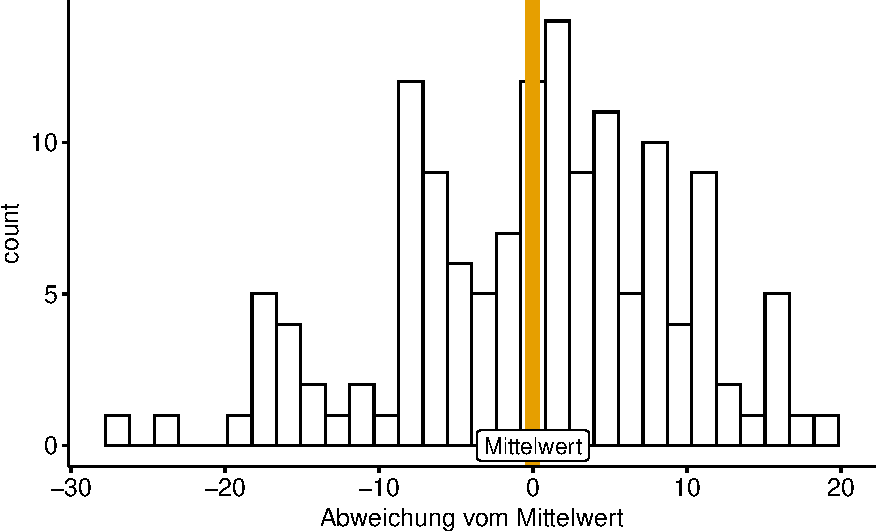
\includegraphics{060-modellguete_files/figure-pdf/fig-mariokart_no_extreme-2.pdf}

}

\subcaption{\label{fig-mariokart_no_extreme-2}Abweichungen vom
Mittelwert: zentrierte Daten}

\end{minipage}%

\caption{\label{fig-mariokart_no_extreme}Verteilung von
\texttt{mariokart\_no\_extreme}}

\end{figure}%

Tja, das ist doch etwas Streuung um den Mittelwert herum.

\begin{tcolorbox}[enhanced jigsaw, opacityback=0, arc=.35mm, left=2mm, colframe=quarto-callout-important-color-frame, toptitle=1mm, colback=white, toprule=.15mm, bottomrule=.15mm, colbacktitle=quarto-callout-important-color!10!white, bottomtitle=1mm, coltitle=black, titlerule=0mm, title=\textcolor{quarto-callout-important-color}{\faExclamation}\hspace{0.5em}{Wichtig}, rightrule=.15mm, breakable, leftrule=.75mm, opacitybacktitle=0.6]

Je weniger Streuung um den Mittelwert (ca. 47 Euro) herum, desto besser
eignet sich der Mittelwert als Modell für die Daten, bzw. desto höher
die Modellgüte.\(\square\)

\end{tcolorbox}

Ja, es ist \emph{etwas} Streuung, aber wie viel? Kann man das genau
angeben? Sie überlegen \ldots{} und überlegen. Da! Eine Idee!

Man könnte vielleicht angeben, wie viel Euro jedes Spiel vom Mittelwert
entfernt ist. Je größer diese Abweichung, desto schlechter die
Modellgüte! Also rechnen Sie diese Abweichung aus.

\begin{Shaded}
\begin{Highlighting}[]
\NormalTok{mariokart\_no\_extreme }\OtherTok{\textless{}{-}}
\NormalTok{  mariokart\_no\_extreme }\SpecialCharTok{\%\textgreater{}\%} 
  \FunctionTok{mutate}\NormalTok{(}\AttributeTok{abw =} \FloatTok{47.4} \SpecialCharTok{{-}}\NormalTok{ total\_pr)}
\end{Highlighting}
\end{Shaded}

Anders gesagt: Wir haben die Verkaufspreise \emph{zentriert.}

\begin{definition}[Zentrieren]\protect\hypertarget{def-zentrieren}{}\label{def-zentrieren}

Zentrieren bedeutet, von jedem Wert einer Verteilung \(X\) den
Mittelwert abzuziehen. Daher ist der neue Mittelwert (der zentrierten
Verteilung) gleich Null. \(\square\)

\end{definition}

\begin{figure}

\centering{

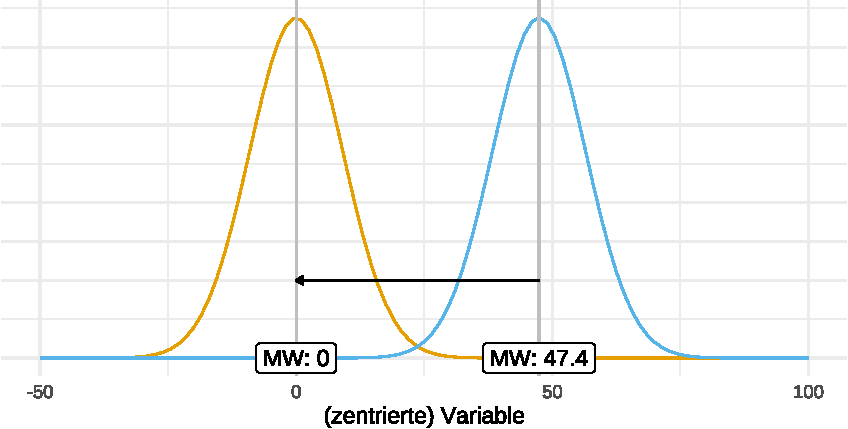
\includegraphics{060-modellguete_files/figure-pdf/fig-norm-dev-1.pdf}

}

\caption{\label{fig-norm-dev}Die Abweichungen zum Mittelwert (MW) einer
normalverteilten Variable sind selber normalverteilt}

\end{figure}%

Aber irgendwie sind Sie noch nicht am Ziel Ihrer Überlegungen: Woher
weiß man, ob 10 Euro oder 20 Euro ``viel'' Abweichung vom Verkaufspreis
ist? Man müsste die Abweichung eines Verkaufpreis zu irgendetwas in
Bezug setzen. Wieder! Ein Geistesblitz! Man könnte doch die jeweilige
Abweichung in Bezug setzen zur \emph{mittleren (absoluten) Abweichung}
(MAA)! Ein alternativer, ähnlicher Kennwert zur mittlerer absolute
Abweichung ist die SD. Sie haben gehört, dass die SD gebräuchlicher ist
als die MAA. Um sich als Checker zu präsentieren, berechnen Sie also
auch die SD; die beiden Koeffizienten sind ja ähnlich.

Also: Wenn ein Spiel 10 Euro vom Mittelwert abweicht und die SD 10 Euro
betragen sollte, dann hätten wir eine ``standardisierte''\footnote{abgekürzt
  manchmal mit \texttt{std}} Abweichung von 1, weil 10/10=1.

Begeistert über Ihre Schlauheit machen Sie sich ans Werk.

\begin{Shaded}
\begin{Highlighting}[]
\NormalTok{mariokart\_no\_extreme }\OtherTok{\textless{}{-}}
\NormalTok{  mariokart\_no\_extreme }\SpecialCharTok{\%\textgreater{}\%} 
  \FunctionTok{mutate}\NormalTok{(}\AttributeTok{abw\_std =}\NormalTok{ abw }\SpecialCharTok{/} \FunctionTok{sd}\NormalTok{(abw),  }\CommentTok{\# std wie "standardisiert"}
         \AttributeTok{abw\_std2 =}\NormalTok{ abw }\SpecialCharTok{/} \FunctionTok{mean}\NormalTok{(}\FunctionTok{abs}\NormalTok{(abw)))  }
\end{Highlighting}
\end{Shaded}

Zufrieden betrachten Sie Ihr Werk, s. Abbildung~\ref{fig-z-transf}. In
Abbildung~\ref{fig-z-transf} sieht man oben die Rohwerte und unten die
transformierten Werte, die wir hier als \emph{standardisiert}
bezeichnen, da wir sie in Bezug zur ``typischen Abweichung'', der SD,
gesetzt haben.

\begin{figure}

\centering{

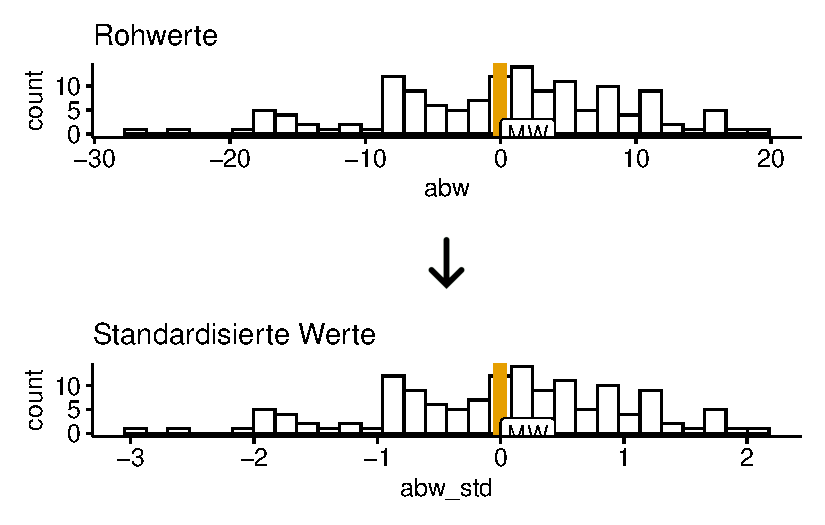
\includegraphics{060-modellguete_files/figure-pdf/fig-z-transf-1.pdf}

}

\caption{\label{fig-z-transf}Standardisierung von Abweichungswerten bzw.
einer Verteilung; der vertikale Balken zeigt den Mittelwert}

\end{figure}%

Wir fassen die Schritte unserer Umrechnung (``Transformation'') zusammen
wie in einem Kochrezept:

\begin{enumerate}
\def\labelenumi{\arabic{enumi}.}
\tightlist
\item
  Nimm die Verteilung der Verkaufspreise
\item
  Berechne die Abweichungen vom mittleren Verkaufspreis (Differenz
  Mittelwert und jeweiliger Verkaufspreis)
\item
  Teile die Abweichungen (Schritt 2) durch die SD
\end{enumerate}

Diese Art von Transformation bezeichnet man als \emph{z-Transformation}
und die resultierenden Werte als \emph{z-Werte}.

\begin{definition}[z-Werte]\protect\hypertarget{def-z-werte}{}\label{def-z-werte}

z-Werte sind das Resultat der z-Transformation. Für die Variable \(X\)
berechnet sich der z-Wert der \(i\)-ten Beobachtung so:
\(z_i = \frac{x_i - \bar{x}}{sd_x}.\square\)

\end{definition}

z-Werte sind nützlich, weil sie die ``relative'' Abweichung einzelner
Beobachtungen vom Mittelwert anzeigen.

Nach einer \emph{Faustregel} spricht man von extremen Abweichungen
(Extremwerten, Ausreißern), wenn \(z_i > 2\) oder \(z_i > 3\).

\section{Fazit}\label{fazit}

Der „gesunde Menschenverstand`` würde spontan den mittleren
Absolutabstand (MAA oder MAE) der Varianz (oder der Standardabweichung,
SD) vorziehen. Das ist vernünftig, denn die MAA ist anschaulicher und
damit nützlicher als die Varianz und die SD.

Warum sollte man überhaupt ein unanschauliches Maß wie die Varianz
verwenden? Wenn es nur um deskriptive Statistik geht, braucht man die
Varianz (oder die SD) nicht unbedingt. Gründe, warum Sie die Varianz
(bzw. SD) kennen und nutzen sollten, sind:\footnote{Ich wollte noch
  hinzufügen, dass die Varianz eng verknüpft mit der linearen Algebra,
  aber ich war nicht sicher, ob das Argument allgemein überzeugen würde.}

\begin{itemize}
\tightlist
\item
  Die SD ist sehr nützlich zur Beschreibung der Normalverteilung
\item
  Die Varianz wird häufig verwendet bzw. in Forschungsarbeiten
  berichtet, also müssen Sie die Varianz kennen.
\end{itemize}

Liegen Extremwerte vor, kann es vorteilhafter sein, den IQR vorzuziehen
gegenüber Mittelwert basierten Streuungsmaßen (MAA, Varianz, SD).

\section{Aufgaben}\label{aufgaben}

\subsection{Datenwerk}\label{datenwerk}

Die Webseite \href{https://datenwerk.netlify.app}{datenwerk.netlify.app}
stellt eine Reihe von einschlägigen Übungsaufgaben bereit. Sie können
die Suchfunktion der Webseite nutzen, um die Aufgaben mit den folgenden
Namen zu suchen:

\begin{itemize}
\tightlist
\item
  \href{https://datenwerk.netlify.app/posts/mariokart-sd2/mariokart-sd2}{mariokart-sd2}
\item
  \href{https://datenwerk.netlify.app/posts/mariokart-sd3/mariokart-sd3}{mariokart-sd3}
\item
  \href{https://datenwerk.netlify.app/posts/kennwert-robust/kennwert-robust}{Kennwert-robust}
\item
  \href{https://datenwerk.netlify.app/posts/summarise04/summarise04}{summarise04}
\item
  \href{https://datenwerk.netlify.app/posts/summarise05/summarise05}{summarise05}
\item
  \href{https://datenwerk.netlify.app/posts/vis-mariokart-variab/vis-mariokart-variab}{vis-mariokart-variab}
\item
  \href{https://datenwerk.netlify.app/posts/sd-vergleich/sd-vergleich}{sd-vergleich}
\item
  \href{https://datenwerk.netlify.app/posts/nasa01/nasa01}{nasa01}
\item
  \href{https://datenwerk.netlify.app/posts/streuung-histogramm/streuung-histogramm}{Streuung-Histogramm}
\item
  \href{https://datenwerk.netlify.app/posts/mariokart-sd1/mariokart-sd1}{mariokart-sd1}
\item
  \href{https://datenwerk.netlify.app/posts/summarise06/summarise06}{summarise06}
\item
  \href{https://datenwerk.netlify.app/posts/mariokart-desk01/mariokart-desk01}{mariokart-desk01}
\end{itemize}

\begin{exercise}[Analysieren Sie den Datensatz zur
Handynutzung]\protect\hypertarget{exr-handy}{}\label{exr-handy}

~

\subsection{Aufgabe}

Sind Sie händysüchtig? Das ist die Forschungsfrage
\href{https://docs.google.com/forms/d/e/1FAIpQLSfM6oDLHX4_lqWq-bXw39drTkdGAvecE6ow2HIKoxdrVygp2A/viewform}{dieser
Umfrage}. Nehmen Sie ggf. an dieser Umfrage teil (sie ist anonym und
dauert drei Minuten). Laden Sie den
\href{https://docs.google.com/spreadsheets/d/1SWMj4rIIIJdAsfsSKQHSg8jHr_OuKLpJx_0XV4LGnH0/edit?usp=sharing}{Datensatz
zur Handynutzung} von Google-Docs herunter.\footnote{\url{https://docs.google.com/spreadsheets/d/1SWMj4rIIIJdAsfsSKQHSg8jHr_OuKLpJx_0XV4LGnH0/edit?usp=sharing}}
Berechnen Sie dann gängige deskriptive Statistiken und visualisieren Sie
sie. \(\square\)

\subsection{Lösung: Daten importieren}

Sie können die Daten entweder selber herunterladen oder aber die
folgende Version des Datensatzes verwenden. In beiden Fällen ist es
nützlich, den (absoluten oder relativen) Pfad anzugeben:

\begin{Shaded}
\begin{Highlighting}[]
\NormalTok{data\_path }\OtherTok{\textless{}{-}} \StringTok{"https://raw.githubusercontent.com/sebastiansauer/statistik1/main/daten/Smartphone{-}Nutzung\%20(Responses)\%20{-}\%20Form\%20responses\%201.csv"}
\end{Highlighting}
\end{Shaded}

Dann können Sie die Daten wie gewohnt importieren:

\begin{Shaded}
\begin{Highlighting}[]
\NormalTok{smartphone\_raw }\OtherTok{\textless{}{-}} \FunctionTok{read.csv}\NormalTok{(data\_path)}
\end{Highlighting}
\end{Shaded}

\subsection{Lösung: Daten aufbereiten}

Die Spaltennamen sind sehr unschön. Lassen Sie uns daher die
Spaltennamen umbenennen (aber vorab sichern):

\begin{Shaded}
\begin{Highlighting}[]
\NormalTok{item\_labels }\OtherTok{\textless{}{-}} \FunctionTok{names}\NormalTok{(smartphone\_raw)}

\FunctionTok{names}\NormalTok{(smartphone\_raw) }\OtherTok{\textless{}{-}} \FunctionTok{paste0}\NormalTok{(}\StringTok{"item"}\NormalTok{,}\DecValTok{1}\SpecialCharTok{:}\FunctionTok{ncol}\NormalTok{(smartphone\_raw))}
\end{Highlighting}
\end{Shaded}

Check:

\begin{Shaded}
\begin{Highlighting}[]
\FunctionTok{glimpse}\NormalTok{(smartphone\_raw)}
\DocumentationTok{\#\# Rows: 70}
\DocumentationTok{\#\# Columns: 18}
\DocumentationTok{\#\# $ item1  \textless{}chr\textgreater{} "21/03/2024 15:36:52", "05/04/2024 10:24:58\textasciitilde{}}
\DocumentationTok{\#\# $ item2  \textless{}chr\textgreater{} "15:31:00", "10:23:00", "10:40:00", "11:14:\textasciitilde{}}
\DocumentationTok{\#\# $ item3  \textless{}int\textgreater{} 3, 4, 3, 3, 5, 5, 5, 5, 1, 2, 5, 3, 2, 2, 2\textasciitilde{}}
\DocumentationTok{\#\# $ item4  \textless{}int\textgreater{} 5, 3, 3, 3, 4, 3, 3, 6, 2, 4, 5, 1, 1, 2, 3\textasciitilde{}}
\DocumentationTok{\#\# $ item5  \textless{}int\textgreater{} 3, 3, 1, 5, 1, 3, 2, 4, 3, 2, 1, 1, 1, 4, 1\textasciitilde{}}
\DocumentationTok{\#\# $ item6  \textless{}int\textgreater{} 4, 2, 4, 3, 5, 4, 6, 3, 2, 5, 6, 4, 2, 6, 5\textasciitilde{}}
\DocumentationTok{\#\# $ item7  \textless{}int\textgreater{} 4, 3, 2, 3, 3, 1, 3, 2, 1, 2, 1, 1, 1, 3, 2\textasciitilde{}}
\DocumentationTok{\#\# $ item8  \textless{}int\textgreater{} 1, 3, 1, 2, 3, 1, 1, 2, 2, 2, 1, 1, 2, 4, 1\textasciitilde{}}
\DocumentationTok{\#\# $ item9  \textless{}int\textgreater{} 2, 6, 1, 3, 6, 5, 5, 2, 2, 5, 6, 1, 1, 5, 4\textasciitilde{}}
\DocumentationTok{\#\# $ item10 \textless{}int\textgreater{} 2, 5, 5, 3, 4, 3, 1, 5, 1, 5, 3, 4, 3, 5, 4\textasciitilde{}}
\DocumentationTok{\#\# $ item11 \textless{}int\textgreater{} 5, 6, 6, 5, 6, 6, 5, 6, 4, 3, 6, 4, 4, 5, 3\textasciitilde{}}
\DocumentationTok{\#\# $ item12 \textless{}int\textgreater{} 1, 3, 1, 2, 5, 2, 4, 2, 1, 1, 3, 1, 1, 1, 1\textasciitilde{}}
\DocumentationTok{\#\# $ item13 \textless{}int\textgreater{} 4, 3, 4, 2, 4, 2, 5, 3, 1, 1, 4, 1, 3, 4, 1\textasciitilde{}}
\DocumentationTok{\#\# $ item14 \textless{}chr\textgreater{} "", "", "", "", "", "", "", "", "", "", "",\textasciitilde{}}
\DocumentationTok{\#\# $ item15 \textless{}chr\textgreater{} "", "", "", "", "", "", "", "", "", "", "",\textasciitilde{}}
\DocumentationTok{\#\# $ item16 \textless{}int\textgreater{} NA, NA, NA, NA, NA, NA, NA, NA, NA, NA, NA,\textasciitilde{}}
\DocumentationTok{\#\# $ item17 \textless{}chr\textgreater{} "", "", "", "", "", "", "", "", "", "", "",\textasciitilde{}}
\DocumentationTok{\#\# $ item18 \textless{}int\textgreater{} NA, NA, NA, NA, NA, NA, NA, NA, NA, NA, NA,\textasciitilde{}}
\end{Highlighting}
\end{Shaded}

\subsection{Lösung: Komplett}

😁

\end{exercise}

\subsection{Fallstudie zur
Lebenszufriedenheit}\label{fallstudie-zur-lebenszufriedenheit}

Die OECD führt eine
\href{https://www.oecd.org/wise/measuring-well-being-and-progress.htm}{weltweite
Studie zur Lebenszufriedenheit} durch.\footnote{https://www.oecd.org/wise/measuring-well-being-and-progress.htm}

Arbeiten Sie die die
\href{https://datenwerk.netlify.app/posts/oecd-yacsda/}{Fallstudie
``OECD Wellbeing''} durch, um ein tieferes Verständnis für die
Lebenszufriedenheit in verschiedenen Ländern der Welt zu bekommen.

\section{Literaturhinweise}\label{literaturhinweise}

Allen Downey (2023) stellt in seinem vergnüglich zu lesenden Buch eine
kurzweilige Einführung in die Statistik vor; auch Streuungsmaße haben
dabei einen Auftritt. Wer mehr ``Lehrbuch-Feeling'' sucht, wird bei
(\textbf{cetinkaya-rundel\_introduction\_2021-1?}) fündig (das Buch ist
online frei verfügbar). Es ist kein Geheimnis, dass Streuungsmaße keine
ganz neuen Themen in der Statistik sind. Aber hey, Oldie is Goldie, ohne
Streuungsmaße geht's nicht. Jedenfalls werden Sie in jedem
Statistik-Lehrbuch, dass Sie in der Bib (oder sonstwo) aus dem Regal
ziehen, fündig werden zu diesem Thema. Die Bücher unterscheiden sich
meist ``nur'' in ihrem Anspruch bzw. der didaktischen Aufmachung; für
alle ist da was dabei.

\section*{Literatur}\label{literatur}
\addcontentsline{toc}{section}{Literatur}

\phantomsection\label{refs}
\begin{CSLReferences}{1}{0}
\bibitem[\citeproctext]{ref-downey_probably_2023}
Downey, Allen. 2023. \emph{Probably Overthinking It: How to Use Data to
Answer Questions, Avoid Statistical Traps, and Make Better Decisions}.
Chicago ; London: The University of Chicago Press.

\bibitem[\citeproctext]{ref-world_economic_forum_future_2020}
Forum, World Economic. 2020. {„The {Future} of {Jobs Report} 2020``}.
CH-1223 Cologny/Geneva Switzerland: World Economic Forum.
\url{https://www3.weforum.org/docs/WEF_Future_of_Jobs_2020.pdf}.

\end{CSLReferences}




\end{document}
